\documentclass[11pt,openany]{article}

\input{ca-preamble}
\usepackage{tcolorbox}
\tcbset{colback=white, arc=5pt}

\definecolor{axiomcolor}{HTML}{a88bfa}
\definecolor{defcolor}{RGB}{52, 152, 219}
\definecolor{procolor}{RGB}{241, 196, 15}
\definecolor{thmcolor}{RGB}{231, 76, 60}
\definecolor{lemcolor}{RGB}{155, 89, 182}
\definecolor{corcolor}{RGB}{46, 204, 113}
\definecolor{execolor}{RGB}{90, 128, 127}

% Define a new command for the custom tcolorbox
\newcommand{\axiombox}[2][]{%
	\begin{tcolorbox}[colframe=axiomcolor, title={\color{white}\bfseries #1}]
		#2
	\end{tcolorbox}
}

\newcommand{\defbox}[2][]{%
	\begin{tcolorbox}[colframe=defcolor, title={\color{white}\bfseries #1}]
		#2
	\end{tcolorbox}
}

\newcommand{\probox}[2][]{%
	\begin{tcolorbox}[colframe=procolor, title={\color{white}\bfseries #1}]
		#2
	\end{tcolorbox}
}

\newcommand{\thmbox}[2][]{%
	\begin{tcolorbox}[colframe=thmcolor, title={\color{white}\bfseries #1}]
		#2
	\end{tcolorbox}
}

\newcommand{\lembox}[2][]{%
	\begin{tcolorbox}[colframe=lemcolor, title={\color{white}\bfseries #1}]
		#2
	\end{tcolorbox}
}
\usepackage{amsthm}

% Define custom theorem styles
\newtheoremstyle{dotless} % Name of the style
{3pt} % Space above
{3pt} % Space below
{\itshape} % Body font
{} % Indent amount
{\bfseries} % Theorem head font
{} % Punctuation after theorem head
{2.5mm} % Space after theorem head
{} % Theorem head spec

\newtheoremstyle{definitionstyle} % Name of the style
{3pt} % Space above
{3pt} % Space below
{} % Body font
{} % Indent amount
{\bfseries} % Theorem head font
{.} % Punctuation after theorem head
{2.5mm} % Space after theorem head
{} % Theorem head spec

% Applying custom styles
%\theoremstyle{dotless}
\newtheorem{theorem}{Theorem} % Theorem environment with section-wise numbering
\newtheorem*{theorem*}{Theorem} % Theorem environment with section-wise numbering
\newtheorem*{lemma*}{Lemma} % Theorem environment with section-wise numbering
\newtheorem*{proposition*}{Proposition} % Theorem environment with section-wise numbering
\newtheorem*{corollary*}{Corollary} % Theorem environment with section-wise numbering
\newtheorem{proposition}[theorem]{Proposition} % Theorem environment with section-wise numbering
\newtheorem{lemma}[theorem]{Lemma} % Lemma shares the counter with theorem
\newtheorem{corollary}[theorem]{Corollary} % Corollary shares the counter with theorem

\theoremstyle{definitionstyle}
\newtheorem*{observation}{\textcolor{magenta}{Observation}}
\newtheorem*{illustration}{\textcolor{teal}{Illustration}}
\newtheorem*{torus}{{\color{red}T}{\color{orange}o}{\color{green!75!black}r}{\color{cyan}u}{\color{violet}s}}
\newtheorem{definition}{Definition} % Definition shares the counter with theorem
\newtheorem{example}{Example} % Example shares the counter with theorem
\newtheorem{exercise}{{Exercise}} % Example shares the counter with theorem
\newtheorem{remark}{Remark} % Remark shares the counter with theorem
\newtheorem*{note}{Note}
\newtheorem*{notation}{Notation}

\newtheorem*{axiom*}{Axiom}
\newtheorem*{definition*}{Definition} % Definition shares the counter with theorem
\newtheorem*{example*}{Example} % Example shares the counter with theorem
\newtheorem*{exercise*}{\textcolor{teal}{Exercise}} % Example shares the counter with theorem
\newtheorem*{remark*}{Remark} % Remark shares the counter with theorem


\usepackage{tikz}
\usepackage{tikz-cd}
\usetikzlibrary{shadows}
\usetikzlibrary{shapes.geometric, arrows.meta, positioning}
\input{ca-commands}
\renewcommand{\Re}{\mathrm{Re}}
\renewcommand{\Im}{\mathrm{Im}}
\renewcommand{\vec}[1]{\mathbf{#1}}
\renewcommand{\emph}[1]{\textbf{#1}}
\renewcommand{\d}{\mathrm{d}} % For the exterior derivative 'd'
\newcommand{\pderiv}[2]{\frac{\partial #1}{\partial #2}}
\newcommand{\spderiv}[3]{\frac{\partial^2 #1}{\partial #2\partial #3}}
\newcommand{\vect}[1]{\begin{bmatrix} #1 \end{bmatrix}}

\renewcommand{\Re}{\operatorname{\mathrm{Re}}}
\renewcommand{\Im}{\operatorname{\mathrm{Im}}}

\newcommand{\circulationsquare}[1]{
	\draw[thick, gray] #1 rectangle ++(1,1);
	\begin{scope}[decoration={markings, mark=at position 0.5 with {\arrow{>}}}]
		\draw[postaction={decorate}, blue] #1 -- ++(1,0);
		\draw[postaction={decorate}, blue] ++(1,0) -- ++(0,1);
		\draw[postaction={decorate}, blue] ++(0,1) -- ++(-1,0);
		\draw[postaction={decorate}, blue] ++(-1,0) -- cycle;
	\end{scope}
}

\newcommand{\Sol}{{\color{magenta}\normalfont\bfseries\text{Sol}}}

\usepackage{esvect}
\usepackage{physics}

\setstretch{1.25}

\begin{document}
	\pagenumbering{arabic}
	\begin{center}
		\huge\textbf{Complex Analysis}\\
		\vspace{0.5em}
		\large{Ji, Yong-hyeon}\\
		\vspace{0.5em}
		\normalsize{\today}\\
	\end{center} 
	%\[\boxed{
		%\underbrace{f}_{\Omega^0}
		%\;\xrightarrow{d}\;
		%\underbrace{df}_{\Omega^1}
		%\;\longleftrightarrow\;
		%\underbrace{\nabla f}_{\substack{\text{gradient}\\\text{vector field}}}
		%\quad
		%\longrightarrow
		%\quad
		%\underbrace{\mathbf F}_{(\Omega^0)^m}
		%\;\xrightarrow{d}\;
		%\underbrace{d\mathbf F}_{\Omega^1\otimes\R^m}
		%\;\longleftrightarrow\;
		%\underbrace{D\mathbf F}_{\substack{\text{Jacobian}\\\text{matrix}}}}
	%\]
%	\noindent 
%	We cover the following topics in this note.
%	\begin{itemize}
%		\item Vector calculus (conservative fields, irrotational field)
%		\item Differential forms (exact forms, closed forms)
%	\end{itemize}
	%In this note, we build a bridge between the familiar concepts of vector calculus (conservative fields, curl) and the language of differential forms (exact forms, closed forms)
	%\hrule\vspace{12pt}
%	\begin{center}
%		\begin{tabular*}{\textwidth}{@{\extracolsep{\fill}} l c l}
%			\hline
%			\textbf{Vector Calculus (in $\R^2$ or $\R^3$)} & & \textbf{Differential Forms} \\
%			\hline
%			Vector Field $\vec F$ & $\iff$ & 1-form $\omega$ \\
%			Conservative Vector Field ($\vec F = \nabla f$) & $\iff$ & Exact 1-form ($\omega = \d f$) \\
%			Irrotational Vector Field ($\nabla \times \vec F = \mathbf{0}$) & $\iff$ & Closed 1-form ($\d\omega = 0$) \\
%			\hline
%		\end{tabular*}
%	\end{center}

\tableofcontents

\vspace{1em}

\newpage
\section{Complex Numbers}

\subsection{Complex Numbers}

\begin{definition}[Complex numbers and parts]
	A complex number is an ordered pair $(x,y)\in\R^2$, denoted $z=(x,y)$ or $z=x+iy$, with \emph{real part} $\Re z=x$ and \emph{imaginary part} $\Im z=y$.
\end{definition}

\begin{remark}
	Two complex numbers are equal iff they have the same real and imaginary parts.
\end{remark}

\begin{definition}[Algebra]
For $z_1=(x_1,y_1)$ and $z_2=(x_2,y_2)$,
\[
z_1+z_2=(x_1+x_2,\,y_1+y_2),\qquad
z_1z_2=(x_1x_2-y_1y_2,\,x_1y_2+y_1x_2).
\]
Let $i=(0,1)$. then $i^2=-1$ and every $z$ can be written $x+iy$.
\end{definition}

\begin{remark}[Basic properties]
	The complex numbers satisfy the usual commutative, associative, and distributive laws; $0=(0,0)$ and $1=(1,0)$ are additive/multiplicative identities. For $z\ne0$, the multiplicative inverse is
	\[
	z^{-1}=\frac{\bar z}{|z|^2}=\frac{x-iy}{x^2+y^2}.
	\]
	If $z_2\ne0$,
	\[
	\frac{z_1}{z_2}=\frac{x_1x_2+y_1y_2}{x_2^2+y_2^2}+i\,\frac{y_1x_2-x_1y_2}{x_2^2+y_2^2}.
	\]
\end{remark}

\begin{definition}[Binomial formula]
	For $n\in\mathbb{N}$ and $z_1,z_2\in\C$,
	\[
	(z_1+z_2)^n=\sum_{k=0}^n \binom{n}{k}\,z_1^{\,k}z_2^{\,n-k}.
	\]
\end{definition}

\subsection{Vectors and Moduli}

\begin{definition}[Modulus and distance]
	For $z=x+iy$, the \emph{modulus} is $|z|=\sqrt{x^2+y^2}$. The distance between $z_1=(x_1,y_1)$ and $z_2=(x_2,y_2)$ is $|z_1-z_2|=\sqrt{(x_1-x_2)^2+(y_1-y_2)^2}$.
\end{definition}

\begin{remark}
	The circle of center $z_0$ and radius $R>0$ is $\{z:|z-z_0|=R\}$.
\end{remark}

\subsection{Complex Conjugation}

\begin{definition}[Conjugate]
	For $z=x+iy$, the \emph{conjugate} is $\bar z=x-iy$.
\end{definition}

\begin{theorem}[Conjugation identities]
	For any $z,z_1,z_2\in\C$ (with $z_2\ne0$),
	\[
	\overline{\bar z}=z,\quad |z|=|\bar z|,\quad
	\overline{z_1\pm z_2}=\bar z_1\pm\bar z_2,\quad
	\overline{z_1z_2}=\bar z_1\,\bar z_2,\quad
	\overline{\frac{z_1}{z_2}}=\frac{\bar z_1}{\bar z_2},
	\]
	\[
	\Re z=\frac{z+\bar z}{2},\quad \Im z=\frac{z-\bar z}{2i},\quad
	|z|^2=z\bar z,
	\quad |z_1z_2|=|z_1||z_2|.
	\]
\end{theorem}

\begin{theorem}[Triangle inequality]
	For all $z_1,z_2\in\C$,
	\[
	|z_1+z_2|\le |z_1|+|z_2|.
	\]
	Consequently, $|z_1+z_2|\ge\big||z_1|-|z_2|\big|$ and for any $n\in\mathbb{N}$,
	\[
	\Big|\sum_{k=1}^n z_k\Big|\le \sum_{k=1}^n |z_k|.
	\]
\end{theorem}

\subsection{Polar and Exponential Form}

\begin{definition}[Polar form, argument]
	For $z\ne0$, write $z=r(\cos\theta+i\sin\theta)=re^{i\theta}$ with $r=|z|$ and any \emph{argument} $\theta\in\arg z=\{\Arg z+2\pi k:k\in\mathbb{Z}\}$, where $\Arg z\in(-\pi,\pi]$ is the principal value. (For $z=0$, $\theta$ is undefined.)
\end{definition}

\begin{definition}[Euler's formula]
	$e^{i\theta}=\cos\theta+i\sin\theta\quad(\theta\in\R)$.
\end{definition}

\begin{remark}[Parametrizing circles]
	The circle $|z|=R$ has parametrization $z=Re^{i\theta}$, $0\le\theta\le2\pi$. The circle $|z-z_0|=R$ has $z=z_0+Re^{i\theta}$.
\end{remark}

\subsection{Products, Powers, and Arguments}

\begin{proposition}[Product/quotient in polar form]
	If $z_j=r_je^{i\theta_j}$ $(j=1,2)$ with $r_j>0$, then
	\[
	z_1z_2=r_1r_2\,e^{i(\theta_1+\theta_2)},\qquad
	\frac{z_1}{z_2}=\frac{r_1}{r_2}\,e^{i(\theta_1-\theta_2)},\qquad
	z^{-1}=\frac{1}{r}\,e^{-i\theta}.
	\]
	For $n\in\mathbb{Z}$, $z^n=r^{\,n}e^{in\theta}$.
\end{proposition}

\begin{corollary}[de Moivre]
	For $n\in\mathbb{Z}$, $(\cos\theta+i\sin\theta)^{n}=\cos(n\theta)+i\sin(n\theta)$.
\end{corollary}

\begin{theorem}[Arguments]
	If $z_j=r_je^{i\theta_j}$ $(j=1,2)$, then $\arg(z_1z_2)=\arg z_1+\arg z_2$ and $\arg\!\left(\frac{z_1}{z_2}\right)=\arg z_1-\arg z_2$ (mod $2\pi$). Using principal values requires care at the branch cut.
\end{theorem}

\subsection{Roots of Complex Numbers}

\begin{theorem}[All $n$th roots]\label{thm:nthroots}
	Let $z_0=r_0e^{i\theta_0}\ne0$ and $n\in\mathbb{N}$. The solutions of $z^n=z_0$ are
	\[
	z_k=\sqrt[n]{r_0}\;\exp\!\left(i\,\frac{\theta_0+2\pi k}{n}\right),\qquad k=0,1,\dots,n-1.
	\]
	These $n$ distinct roots lie on the circle $|z|=\sqrt[n]{r_0}$ at equal angular spacing $2\pi/n$. The root with $k=0$ (when $\theta_0=\Arg z_0$) is the \emph{principal root}.
\end{theorem}

\begin{remark}[Roots of unity]
	For $z_0=1$, the $n$th roots are $e^{2\pi i k/n}$, $k=0,\dots,n-1$.
\end{remark}

\begin{example}[Cube roots of $-8i$]
	Since $-8i=8\,e^{-i\pi/2}$, the cube roots are $2\,e^{i(-\pi/6+2\pi k/3)}$, $k=0,1,2$.
\end{example}

\subsection{Regions in the Complex Plane}

\begin{definition}[Neighborhoods]
	An $\varepsilon$-neighborhood of $z_0$ is $\{z:|z-z_0|<\varepsilon\}$. The \emph{deleted} (punctured) neighborhood is $\{z:0<|z-z_0|<\varepsilon\}$.
\end{definition}

\begin{definition}[Interior, exterior, boundary]
	A point $z_0$ is an interior point of $S$ if some neighborhood of $z_0$ lies in $S$; an exterior point if some neighborhood lies in $S^{c}$; otherwise $z_0$ is on the boundary $\partial S$.
\end{definition}

\begin{definition}[Open/closed, closure]
	A set is \emph{open} if it contains none of its boundary points; \emph{closed} if it contains all of them. The \emph{closure} $\overline{S}$ is $S\cup\partial S$.
\end{definition}

\begin{definition}[Connected, domain, region]
	An open set $S$ is \emph{connected} if any two points can be joined by a polygonal line lying in $S$. A nonempty connected open set is a \emph{domain}. A \emph{region} is a domain together with some (possibly all or none) of its boundary points.
\end{definition}

\begin{definition}[Boundedness]
	$S$ is \emph{bounded} if $S\subset\{z:|z|<R\}$ for some $R>0$.
\end{definition}

\begin{definition}[Accumulation points]
	A point $z_0$ is an accumulation point of $S$ if every deleted neighborhood of $z_0$ contains a point of $S$. A set is closed iff it contains all its accumulation points.
\end{definition}

\newpage
\subsection{Exercises}
\begin{enumerate}[\bfseries 1.]
\item Verify that $\sqrt{2}\,|z|\ge |\Re z|+|\Im z|$.
\begin{proof}[\Sol]
Let $z=x+iy$, so that $x=\Re z$, $y=\Im z$, and $\lvert z\rvert=\sqrt{x^2+y^2}$. Then
\begin{align*}
\sqrt{2}\,\lvert z\rvert \;\ge\; \lvert \Re z\rvert+\lvert \Im z\rvert&\iff\sqrt{2}\,\sqrt{x^2+y^2}\;\ge\;\lvert x\rvert+\lvert y\rvert\\
&\iff 2(x^2+y^2)\;\ge\;(\lvert x\rvert+\lvert y\rvert)^2\\
&\iff 2(x^2+y^2)\;\ge\;x^2+y^2+2\lvert x\rvert\lvert y\rvert\quad(\because |x|^2=x^2,\; |y|^2=y^2)\\
&\iff x^2+y^2\;\ge\;2\lvert x\rvert\lvert y\rvert\quad\text{by subtracting $x^2+y^2$ from both sides}\\
&\iff x^2+y^2\;\ge\;2\sqrt{x^2y^2} \\
&\iff \frac{x^2+y^2}{2}\;\ge\;\sqrt{x^2y^2} \\
&\iff \frac{a+b}{2}\;\ge\;\sqrt{ab}\quad\text{by setting $a:=x^2$ and $b:=y^2$;\quad (AM-GM inequality)} \\
\end{align*}
Hence it holds.
\begin{center}
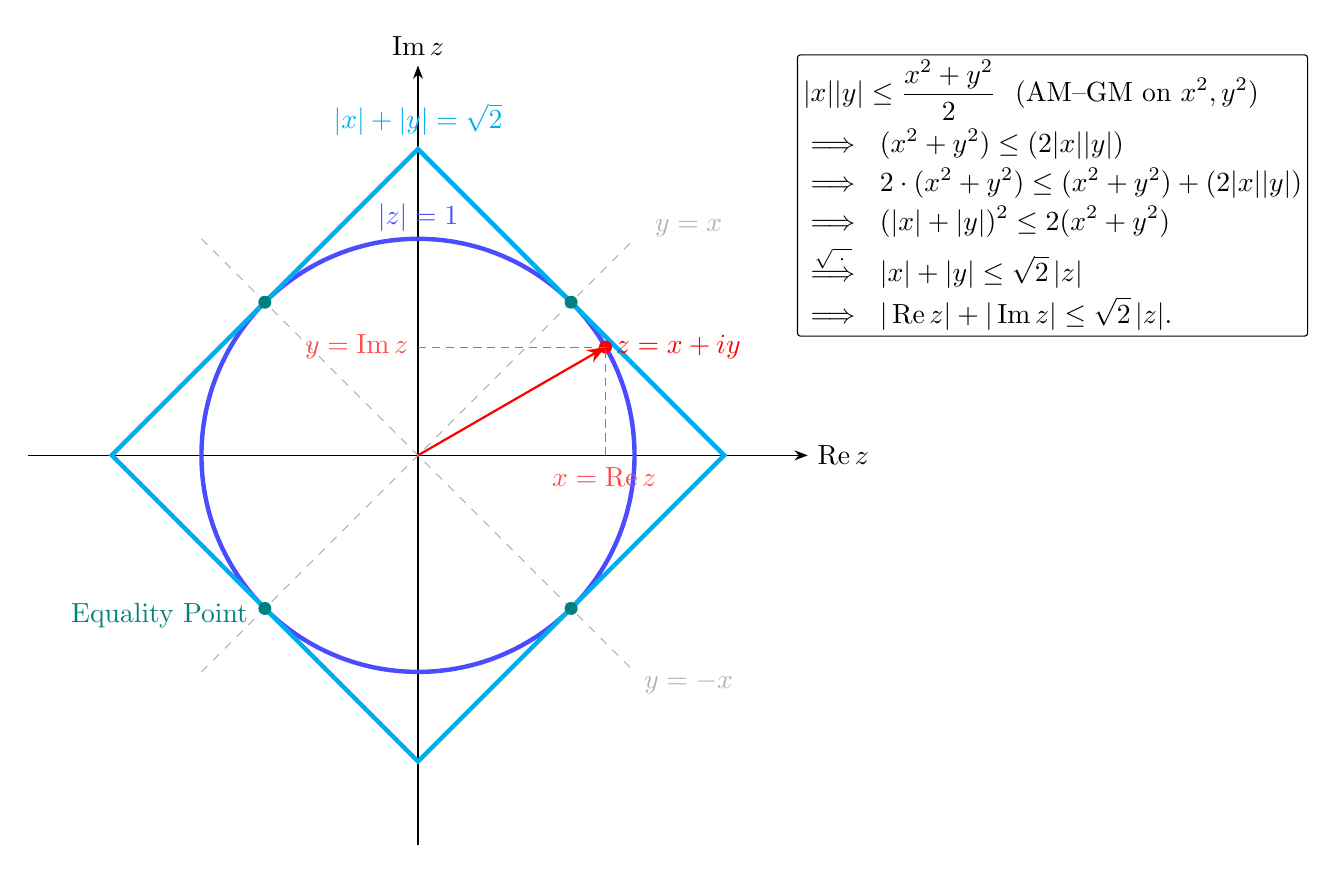
\begin{tikzpicture}[scale=2.75, >=Stealth]
	% axes
	\draw[->] (-1.8,0) -- (1.8,0) node[right] {$\Re z$};
	\draw[->] (0,-1.8) -- (0,1.8) node[above] {$\Im z$};
	
	% unit circle |z|=1
	\draw[ultra thick,blue!70] (0,0) circle (1);
%	\draw[ultra thick,blue!70, opacity=.5] (0,0) circle (0.7207);
	\node[blue!70] at (0,1.1) {$|z|=1$};
	
	% diamond |x|+|y|=sqrt(2)  (vertices at (±√2,0),(0,±√2))
	% use √2 ≈ 1.4142
	\draw[ultra thick,cyan] ( 1.4142,0) -- (0, 1.4142) -- (-1.4142,0) -- (0,-1.4142) -- cycle;
	\node[cyan] at (0,1.55) {$|x|+|y|=\sqrt{2}$};
	
	% equality rays y=±x
	\draw[dashed,gray!60] (-1,-1) -- (1,1);
	\draw[dashed,gray!60] (-1, 1) -- (1,-1);
	\node[gray!60] at (1.25,1.05) {$y=x$};
	\node[gray!60] at (1.25,-1.05) {$y=-x$};
	
	\foreach \X/\Y in {0.7071/0.7071, 0.7071/-0.7071, -0.7071/0.7071, -0.7071/-0.7071}{
		\fill[teal] (\X,\Y) circle (0.03);
	}
	\node[teal,anchor=east] at (-0.74,-0.74) {Equality Point
%		$\bigl(\tfrac{1}{\sqrt2},\tfrac{1}{\sqrt2}\bigr)$
	};
	
	% a sample point on the circle (theta = 30°)
	% coordinates: (cos 30°, sin 30°) ≈ (0.8660, 0.5)
	\fill[red] (0.8660,0.5000) circle (0.03);
	\draw[red,->,thick] (0,0) -- (0.8660,0.5000) node[right] {$z=x+iy$};
	
	% helper projections to visualize |x| and |y|
	\draw[red!70,densely dashed] (0.8660,0) -- (0.8660,0.5000);
	\draw[red!70,densely dashed] (0,0.5000) -- (0.8660,0.5000);
	\node[red!70] at (0.86,-0.10) {$x=\Re z$};
	\node[red!70, left] at (0,0.50) {$y=\Im z$};
	
	% AM-GM derivation (compact)
	\node[align=left,draw,rounded corners=1pt,inner sep=2pt,anchor=west] at (1.75,1.2)
	{$\displaystyle |x||y|\le\frac{x^2+y^2}{2}\ \ (\text{AM--GM on }x^2,y^2)$\\[2pt]
		$\displaystyle \implies\ (x^2+y^2)\le (2|x||y|)$\\[2pt]
		$\displaystyle \implies\ 2\cdot (x^2+y^2)\le(x^2+y^2)+(2|x||y|)$\\[2pt]
		$\displaystyle \implies\ (|x|+|y|)^2\le 2(x^2+y^2)$\\[2pt]
		$\displaystyle \overset{\sqrt{\;\cdot\;}}{\implies}\ |x|+|y|\le \sqrt{2}\,|z|$\\[2pt]
		$\displaystyle \implies\ |\Re z|+|\Im z|\le \sqrt{2}\,|z|.$};
\end{tikzpicture}
\end{center}
\end{proof}
\item By factoring $z^4-4z+3$ into two quadratic factors show that if $z$ lies on the circle $|z|=2$, then \[
\left|\frac{1}{z^4-4z^2+3}\right|\le \frac13.
\]
\begin{proof}[\Sol]
Since $z^4-4z^2+3 \;=\; (z^2-1)(z^2-3)$, we have \[
\left\lvert z^4-4z^2+3 \right\rvert
= \lvert z^2-1\rvert\,\lvert z^2-3\rvert.
\]
For $\lvert z\rvert=2$ one has $\lvert z^2\rvert=\lvert z\rvert^2=4$. By the triangle inequality,
\[
\lvert z^2-1\rvert \;\ge\; \bigl|\,\lvert z^2\rvert-\lvert 1\rvert\,\bigr| = \lvert 4-1\rvert = 3,
\qquad
\lvert z^2-3\rvert \;\ge\; \bigl|\,\lvert z^2\rvert-\lvert 3\rvert\,\bigr| = \lvert 4-3\rvert = 1.
\]
Hence
\[
\lvert z^4-4z^2+3\rvert \;\ge\; 3\cdot 1 \;=\; 3,
\]
and therefore
\[
\left\lvert\frac{1}{z^4-4z^2+3}\right\rvert \;=\; \frac{1}{\lvert z^4-4z^2+3\rvert} \;\le\; \frac{1}{3}.
\]

\begin{center}
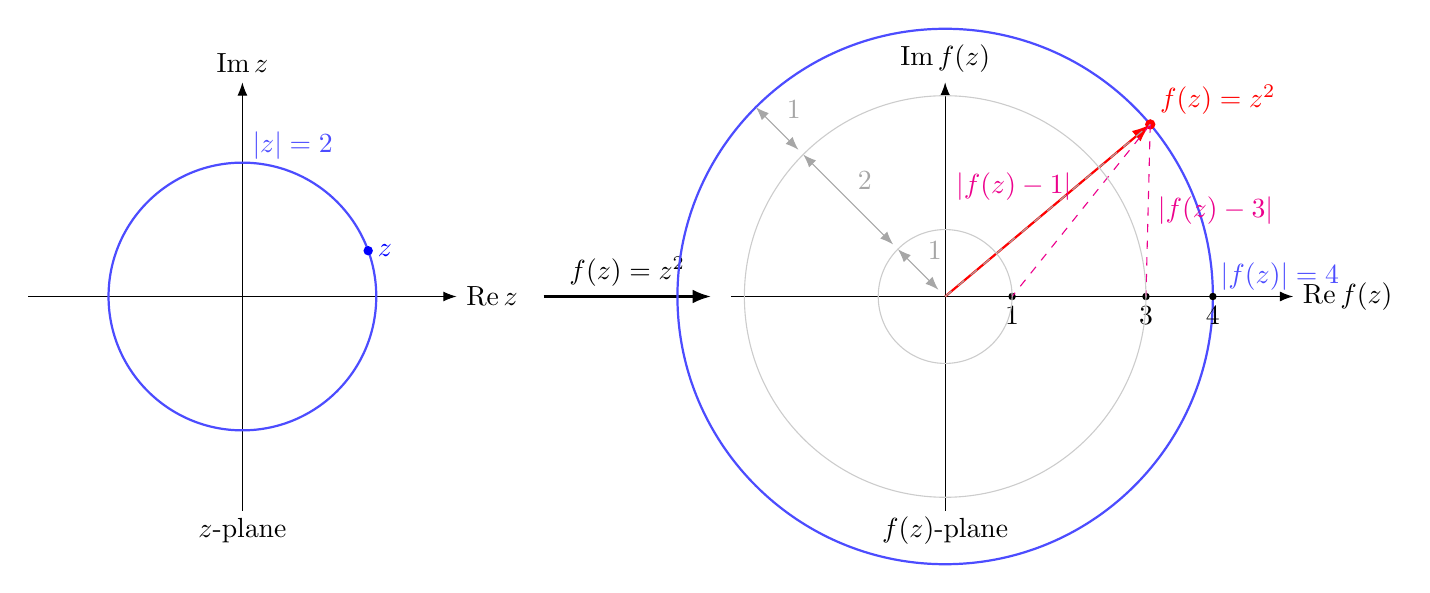
\begin{tikzpicture}[>=Latex,scale=.85]
	
	%================ z-plane =================
	\begin{scope}
		% axes
		\draw[->] (-3.2,0) -- (3.2,0) node[right] {$\Re z$};
		\draw[->] (0,-3.2) -- (0,3.2) node[above] {$\Im z$};
		\node at (0,-3.5) {$z$-plane};
		
		% circle |z|=2
		\draw[thick,blue!70] (0,0) circle (2);
		\node[blue!70] at (0.75,2.25) {$|z|=2$};
		
		% sample point z with |z|=2, angle ~20°
		% coordinates: 2*(cos20, sin20) ≈ (1.8794, 0.6840)
		\fill[blue] (1.8794,0.6840) circle (2pt)
		node[anchor=west] {$z$};
		
		% mapping arrow
		\draw[->,thick] (4.5,0) -- (7,0) node[midway,above] {$f(z)=z^2$};
	\end{scope}
	
	%================ w-plane =================
	\begin{scope}[xshift=10.5cm]
		% axes
		\draw[->] (-3.2,0) -- (5.2,0) node[right] {$\Re f(z)$};
		\draw[->] (0,-3.2) -- (0,3.2) node[above] {$\Im f(z)$};
		\node at (0,-3.5) {$f(z)$-plane};
		
		% circle |w|=4
		\draw[thick,blue!70] (0,0) circle (4);
		\node[blue!70] at (5,0.3) {$|f(z)|=4$};
		
		% two real points 1 and 3
		\fill (1,0) circle (1.6pt) node[below] {$1$};
		\fill (3,0) circle (1.6pt) node[below] {$3$};;
		\fill (4,0) circle (1.6pt) node[below] {$4$};
		
		% image point w = z^2 (angle doubles: ~40°), coords 4*(cos40, sin40) ≈ (3.0640, 2.5712)
		\fill[red] (3.0640,2.5712) circle (2.2pt) node[above right] {$f(z)=z^2$};
		\draw[red,->,thick] (0,0) -- (3.0640,2.5712);
		
		% distances |w-1| and |w-3|
		\draw[magenta, dashed] (3.0640,2.5712) -- (1,0) node[midway,above left] {$|f(z)-1|$};
		\draw[magenta, dashed] (3.0640,2.5712) -- (3,0) node[midway,right] {$|f(z)-3|$};
		
		% triangle-inequality lower bounds along the radial (origin->w) direction
		% show the radial segment length 4, and compare to 1 and 3
		\draw[dashed,gray!70] (0,0) -- (3.0640,2.5712); % radius 4
		% project the points 1 and 3 to the radial line via concentric circles
		\draw[gray!40] (0,0) circle (1);
		\draw[gray!40] (0,0) circle (3);
		
		% double-arrows indicating |4-1|=3 and |4-3|=1 on the radial line
		% place them near the ray with small offsets for clarity
		% marker for 0->1
		\draw[<->,gray!70] (-0.10,0.10) -- (-0.7071,0.7071)
		node[midway,above right] {$1$};
		% marker for 1->3
		\draw[<->,gray!70] (-0.7771,0.7771) -- (-2.1213,2.1213)
		node[midway,above right] {$2$};
		% marker for 3->4
		\draw[<->,gray!70] (-2.1913,2.1913) -- (-2.8284,2.8284)
		node[midway,above right] {$1$};
%		% marker for 0->4 (whole radius)
%		\node[gray!70] at (-1.9,1.2) {$|w|=4$};
		
%		% inequality reminders near the base points
%		\node[align=left,gray!60] at (0.9,1.3)
%		{$|w-1| \ge \bigl||w|-1\bigr|=3$};
%		\node[align=left,gray!60] at (2.6,-1.1)
%		{$|w-3| \ge \bigl||w|-3\bigr|=1$};
		
%		% product and reciprocal bounds
%		\node[draw,rounded corners=2pt,align=left,anchor=west] at (-3.0,-2.4)
%		{$\displaystyle |(w-1)(w-3)| \ge 3\cdot1=3$\\[4pt]
%			$\displaystyle \left|\frac{1}{(w-1)(w-3)}\right| \le \frac{1}{3}$};
	\end{scope}
	
\end{tikzpicture}
\end{center}

For equality in the reverse triangle inequalities we must have $z^2$ and the positive reals $1,3$ on the same ray from the origin, i.e.\ $z^2=4$. Together with $\lvert z\rvert=2$ this forces $z=\pm 2$, and indeed
\[
\lvert (\pm 2)^4 - 4(\pm 2)^2 + 3\rvert = \lvert 16-16+3\rvert = 3,
\]
so the bound is sharp precisely at $z=\pm 2$.
\end{proof}

\item Prove the finite geometric sum
\[
1+z+z^2+\cdots+z^n=\frac{1-z^{n+1}}{1-z}\quad(z\ne1)
\]
and deduce Lagrange's trigonometric identity
\[
1+\cos\theta+\cdots+\cos n\theta=\frac12+\frac{\sin\!\big((2n+1)\theta/2\big)}{2\sin(\theta/2)}\quad(0<\theta<2\pi).
\]
\newpage
\item Prove that the usual formula solves the quadratic equation \[
az^2+bz+c=0\quad (a\neq 0)
\] when the coefficient $a$,$b$, and $c$ are complex numbers. Specifically, by completing the square on the left-hand side, derive the \textbf{quadratic formula} \[
z=\frac{-b+\sqrt{b^2-4ac}}{2a},
\] where both square roots are to be considered when $b^2-4ac\neq 0$. Use this result to find the roots of the equation \[
z^2+2z+(1-i)=0.
\]
\begin{proof}[\Sol]
Since  \[
az^2+bz+c
= a\!\left(z^2+\frac{b}{a}z\right)+c
= a\!\left(z+\frac{b}{2a}\right)^{\!2}-a\!\left(\frac{b}{2a}\right)^{\!2}+c
= a\!\left(z+\frac{b}{2a}\right)^{\!2}-\frac{b^2}{4a}+c,
\] we have
\[
a\!\left(z+\frac{b}{2a}\right)^{\!2}=\frac{b^2}{4a}-c
\quad\Longleftrightarrow\quad
\left(z+\frac{b}{2a}\right)^{\!2}=\frac{b^2-4ac}{4a^2}.
\]
Taking square roots of both sides yields \[
z+\frac{b}{2a}=\pm\,\frac{\sqrt{\,b^2-4ac\,}}{2a},\quad\text{whence}\quad z=\frac{-b\pm\sqrt{\,b^2-4ac\,}}{2a}.
\] Consider $z^2+2z+(1-i)$ with \(a=1\), \(b=2\), and \(c=1-i\). The discriminant is \[
\Delta=b^2-4ac=4-4(1-i)=4i.
\] Since \[
\sqrt{i}=\frac{1+i}{\sqrt{2}}\quad\left(\text{indeed},\; \left(\frac{1+i}{\sqrt{2}}\right)^2=\frac{1+2i-1}{2}=i\right),
\] we may take $\sqrt{\Delta}=\sqrt{4i}=2\sqrt{i}= \sqrt{2}\,(1+i)$.
Therefore \[
z=\frac{-2\pm \sqrt{4i}}{2}
= -1 \pm \sqrt{i}
= -1 \pm \frac{1+i}{\sqrt{2}}.
\] Thus the roots are \[
z_1=-1+\frac{1+i}{\sqrt{2}},
\qquad
z_2=-1-\frac{1+i}{\sqrt{2}}.
\] Note that $z_1,z_2$ are roots of $(z+1)^2=i$.

\begin{center}
\begin{tikzpicture}[>=Latex, scale=4.0]
	% Axes
	\draw[->] (-2.2,0) -- (1.2,0) node[right] {$\Re z$};
	\draw[->] (0,-1.2) -- (0,1.2) node[above] {$\Im z$};
	% Center at -1 + 0i (from completing the square: (z+1)^2 = i)
	\fill (-1,0) circle (0.02) node[below] {$-1$};
	\draw[gray!60] (0,0) circle (1);
	\draw[blue,->, ultra thick] (0,0) -- (0.7071,0.7071)
	node[above right] {$\sqrt{i}=\dfrac{1+i}{\sqrt2}$};
	\filldraw[blue] (0.7071,0.7071) circle (.75pt);
	\node[blue] at (0.45,0.18) {$\arg=\tfrac{\pi}{4}$};
	\draw[cyan,->, ultra thick] (0,0) -- (0,1)
	node[left] {$i=(\sqrt{i})^2$};
	\filldraw[cyan] (0,1) circle (.75pt);
	\node[cyan] at (.2,0.8) {$\arg=\tfrac{\pi}{2}$};
	\draw[teal,->,ultra thick] (0,0) -- (-.7071,-.7071);
	% Roots as endpoints on the circle
	\fill[teal] (-.7071,-.7071) circle (0.03)
	node[below left] {$-\dfrac{1+i}{\sqrt2}$};
	\node[teal] at (-.45,-.18) {$\arg=-\tfrac{\pi}{4}$};
\begin{scope}[yshift=-2.75cm]
% Axes
\draw[->] (-2.2,0) -- (1.2,0) node[right] {$\Re z$};
\draw[->] (0,-1.2) -- (0,1.2) node[above] {$\Im z$};
% Center at -1 + 0i (from completing the square: (z+1)^2 = i)
\node[above, red] at (-1,.25) {$(z+1)^2 = i$};
\fill (-1,0) circle (0.02) node[below] {$-1$};
% Guide: circle of radius 1/sqrt(2) centered at -1
% 1/sqrt(2) ≈ 0.7071
%\draw[gray!60] (-1,0) circle (0.7071);
\draw[gray!60] (-1,0) circle (1);
\draw[gray!60] (0,0) circle (1);
%\node[gray!60] at (-0.35,0.12) {$r=\tfrac{1}{\sqrt2}$};
% Direction line for sqrt(i): 45 degrees through the center (-1,0)
\draw[dashed,gray!60] (-1-1.2,-1.2) -- (-1+1.2,1.2);
%\node[gray!60] at (-0.35,0.58) {$\arg=\tfrac{\pi}{4}$};
\node[blue] at (0.45,0.18) {$\arg=\tfrac{\pi}{4}$};
% The vector sqrt(i) drawn at the origin (reference)
\draw[blue,->,thick] (0,0) -- (0.7071,0.7071)
node[above right] {$\sqrt{i}=\dfrac{1+i}{\sqrt2}$};
%\node[blue] at (0.22,0.18) {$\tfrac{1}{\sqrt2}$};
% Same vector translated to start at -1 (to locate z1)
\draw[blue,->,thick] (-1,0) -- (-0.2929,0.7071);
% Opposite direction (to locate z2)
\draw[blue,->,thick] (-1,0) -- (-1.7071,-0.7071);
% Roots as endpoints on the circle
\fill[red] (-0.2929, 0.7071) circle (0.03)
node[above right] {$z_1=-1+\dfrac{1+i}{\sqrt2}$};
\fill[red] (-1.7071,-0.7071) circle (0.03)
node[below left] {$z_2=-1-\dfrac{1+i}{\sqrt2}$};
\end{scope}
\end{tikzpicture}
\end{center}

\end{proof}

\newpage
\item Determine the accumulation points of each sequence: \[
z_n=i^n,\quad, z_n=\frac{i^n}{n},\quad z_n=(-1)^n(1+i)\frac{n-1}{n}.
\]

\begin{proof}[\Sol]
	content...
\end{proof}
\item Prove that a finite set of points $z_1,z_2,\cdots, z_n$ cannot have any accumulation points.
\begin{proof}[\Sol]
Recall that $w\in\mathbb{C}$ is an accumulation point of $F$ iff for every $\varepsilon>0$ the punctured ball
$B(w,\varepsilon)\setminus\{w\}$ intersects $F$ (equivalently, $B(w,\varepsilon)$ contains a point of $F$ distinct from $w$).

Fix $w\in\mathbb{C}$. Consider the finite set of distances
\[
D:=\{\lvert w-z_k\rvert : 1\le k\le n\}\subset[0,\infty).
\]
Let $d:=\min D$. There are two cases.

\smallskip
\emph{Case 1: $w\notin F$.} Then $d>0$. For $\varepsilon:=\tfrac{d}{2}$ we have
$B(w,\varepsilon)\cap F=\varnothing$, hence $w$ is not an accumulation point.

\smallskip
\emph{Case 2: $w=z_j$ for some $j$.} If $n=1$, then $F=\{w\}$ and for any $\varepsilon>0$ small enough,
$B(w,\varepsilon)\cap(F\setminus\{w\})=\varnothing$, so $w$ is not an accumulation point. If $n\ge2$, put
\[
d':=\min_{k\neq j}\lvert z_j-z_k\rvert \;>\;0
\]
(since the minimum of finitely many positive numbers is positive). For $\varepsilon:=\tfrac{d'}{2}$ we have
$B(w,\varepsilon)\cap(F\setminus\{w\})=\varnothing$, so again $w$ is not an accumulation point.

\smallskip
Since \emph{no} $w\in\mathbb{C}$ can be an accumulation point of $F$, the set $F$ has no accumulation points.

\end{proof}
\end{enumerate}


\begin{definition}
	Let $(z_n)_{n\ge1}$ be a sequence in $\mathbb{C}$. A point $w\in\mathbb{C}$ is an \emph{accumulation point} (or \emph{subsequential limit}) of $(z_n)$ if there exists a strictly increasing map $k\mapsto n_k$ such that $\lim_{k\to\infty} z_{n_k}=w$.
\end{definition}

\begin{enumerate}
	\item[\textbf{(1)}] \(\displaystyle z_n=i^n.\)
	
	\emph{Claim.} The set of accumulation points is \(\{1,i,-1,-i\}\).
	
	\emph{Proof.} Since $i^n$ is $4$-periodic, the image set is $S:=\{1,i,-1,-i\}$, and each element of $S$ occurs infinitely many times. Hence for each $s\in S$ there exists the constant subsequence $z_{n_k}\equiv s$, so $s$ is an accumulation point. Conversely, any subsequence takes all its values in the finite set $S$, thus has a further constant subsequence by the pigeonhole principle; hence every accumulation point lies in $S$. Therefore the accumulation set equals $S$.
	
	\smallskip
	
	\item[\textbf{(2)}] \(\displaystyle z_n=\frac{i^n}{n}.\)
	
	\emph{Claim.} The only accumulation point is \(0\).
	
	\emph{Proof.} Since $\lvert i^n\rvert=1$ for all $n$, we have
	\[
	\lvert z_n\rvert=\frac{1}{n}\xrightarrow[n\to\infty]{}0.
	\]
	Thus $z_n\to 0$, and a convergent sequence has the singleton set $\{0\}$ as its accumulation set.
	
	\smallskip
	
	\item[\textbf{(3)}] \(\displaystyle z_n=(-1)^n(1+i)\,\frac{n-1}{n}.\)
	
	\emph{Claim.} The accumulation points are \(\{\,1+i,\,-(1+i)\,\}\).
	
	\emph{Proof.} Decompose into even/odd subsequences. For $n=2m$,
	\[
	z_{2m}=(1+i)\,\frac{2m-1}{2m}\xrightarrow[m\to\infty]{}1+i.
	\]
	For $n=2m+1$,
	\[
	z_{2m+1}=-(1+i)\,\frac{2m}{2m+1}\xrightarrow[m\to\infty]{}-(1+i).
	\]
	Hence $1+i$ and $-(1+i)$ are accumulation points. If $w$ is an accumulation point, then there exists $n_k\to\infty$ with $z_{n_k}\to w$. Since $\frac{n_k-1}{n_k}\to 1$ and $(-1)^{n_k}\in\{\pm1\}$, every limit $w$ must belong to $\{\pm(1+i)\}$. Thus the accumulation set is exactly $\{\,1+i,\,-(1+i)\,\}$.
\end{enumerate}

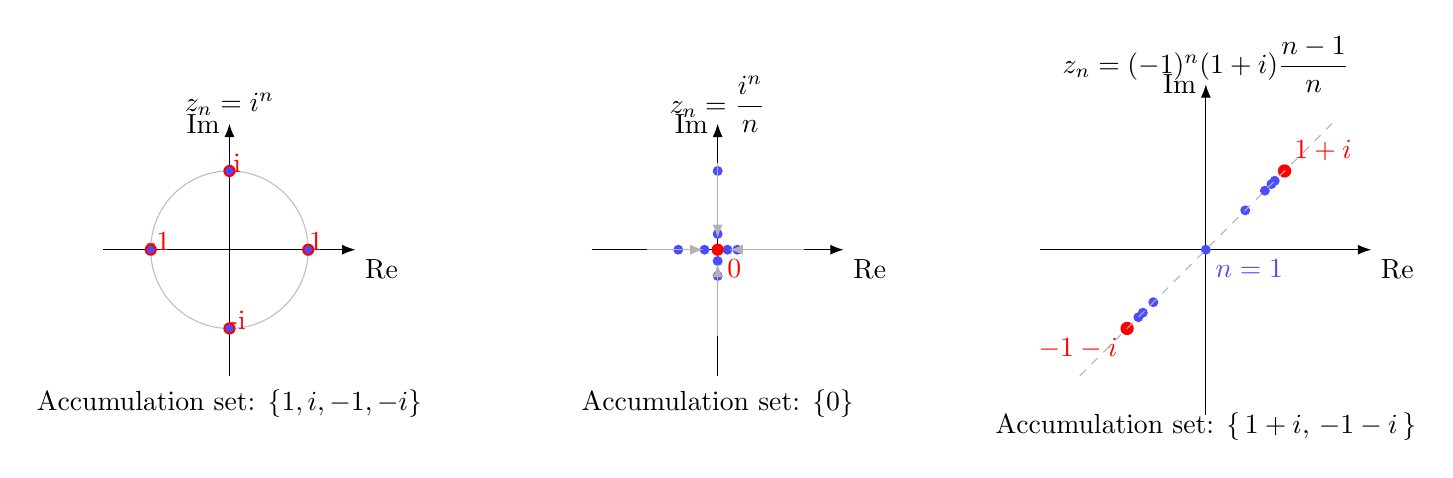
\begin{tikzpicture}[>=Latex,scale=1]
	
	% ================= Panel 1: z_n = i^n =================
	\begin{scope}
		% axes
		\draw[->] (-1.6,0) -- (1.6,0) node[below right] {$\Re$};
		\draw[->] (0,-1.6) -- (0,1.6) node[left] {$\Im$};
		\node at (0,1.85) {$z_n=i^n$};
		
		% unit circle (for context)
		\draw[gray!50] (0,0) circle (1);
		
		% the 4 accumulation points
		\foreach \X/\Y/\L in {1/0/{1}, 0/1/{i}, -1/0/{-1}, 0/-1/{-i}}{
			\fill[red] (\X,\Y) circle (2.2pt) node[shift={(0.1,0.1)}] {\L};
		}
		
		% a few terms n=0..7 to show cycling
		\foreach \P in {(1,0),(0,1),(-1,0),(0,-1),(1,0),(0,1),(-1,0),(0,-1)}{
			\fill[blue!70] \P circle (1.4pt);
		}
		
		\node[align=center] at (0,-1.95) {Accumulation set: $\{1,i,-1,-i\}$};
	\end{scope}
	
	% ================= Panel 2: z_n = i^n / n =================
	\begin{scope}[xshift=6.2cm]
		% axes
		\draw[->] (-1.6,0) -- (1.6,0) node[below right] {$\Re$};
		\draw[->] (0,-1.6) -- (0,1.6) node[left] {$\Im$};
		\node at (0,1.85) {$z_n=\dfrac{i^n}{n}$};
		
		% sample terms n=1..8:
		% (0,1),(-1/2,0),(0,-1/3),(1/4,0),(0,1/5),(-1/6,0),(0,-1/7),(1/8,0)
		\foreach \X/\Y in {0/1, -0.5/0, 0/-0.3333, 0.25/0, 0/0.2, -0.1667/0, 0/-0.1429, 0.125/0}{
			\fill[blue!70] (\X,\Y) circle (1.8pt);
		}
		
		% target 0
		\fill[red] (0,0) circle (2.2pt) node[below right] {$0$};
		
		% hint arrows
		\draw[->,gray!60] (0,1.1) -- (0,0.15);
		\draw[->,gray!60] (-0.9,0) -- (-0.18,0);
		\draw[->,gray!60] (0,-1.1) -- (0,-0.18);
		\draw[->,gray!60] (1.1,0) -- (0.15,0);
		
		\node[align=center] at (0,-1.95) {Accumulation set: $\{0\}$};
	\end{scope}
	
	% ================= Panel 3: z_n = (-1)^n(1+i)(n-1)/n =================
	\begin{scope}[xshift=12.4cm]
		% axes
		\draw[->] (-2.1,0) -- (2.1,0) node[below right] {$\Re$};
		\draw[->] (0,-2.1) -- (0,2.1) node[left] {$\Im$};
		\node at (0,2.35) {$z_n=(-1)^n(1+i)\dfrac{n-1}{n}$};
		
		% limit points at ±(1,1)
		\fill[red] (1,1) circle (2.4pt) node[above right] {$1+i$};
		\fill[red] (-1,-1) circle (2.4pt) node[below left] {$-1-i$};
		
		% terms n=1..8
		% n=1: 0
		\fill[blue!70] (0,0) circle (1.8pt) node[below right] {$n=1$};
		% n even:  (s,s),  s=(n-1)/n = 1-1/n
		% n odd:  (-s,-s)
		% n=2: s=1/2
		\fill[blue!70] (0.5,0.5) circle (1.8pt);
		% n=3: s=2/3
		\fill[blue!70] (-0.6667,-0.6667) circle (1.8pt);
		% n=4: s=3/4
		\fill[blue!70] (0.75,0.75) circle (1.8pt);
		% n=5: s=4/5
		\fill[blue!70] (-0.8,-0.8) circle (1.8pt);
		% n=6: s=5/6
		\fill[blue!70] (0.8333,0.8333) circle (1.8pt);
		% n=7: s=6/7
		\fill[blue!70] (-0.8571,-0.8571) circle (1.8pt);
		% n=8: s=7/8
		\fill[blue!70] (0.875,0.875) circle (1.8pt);
		
		% guide: dashed diagonal where the points lie
		\draw[dashed,gray!60] (-1.6,-1.6) -- (1.6,1.6);
		
		\node[align=center] at (0,-2.25) {Accumulation set: $\{\,1+i,\,-1-i\,\}$};
	\end{scope}
	
\end{tikzpicture}

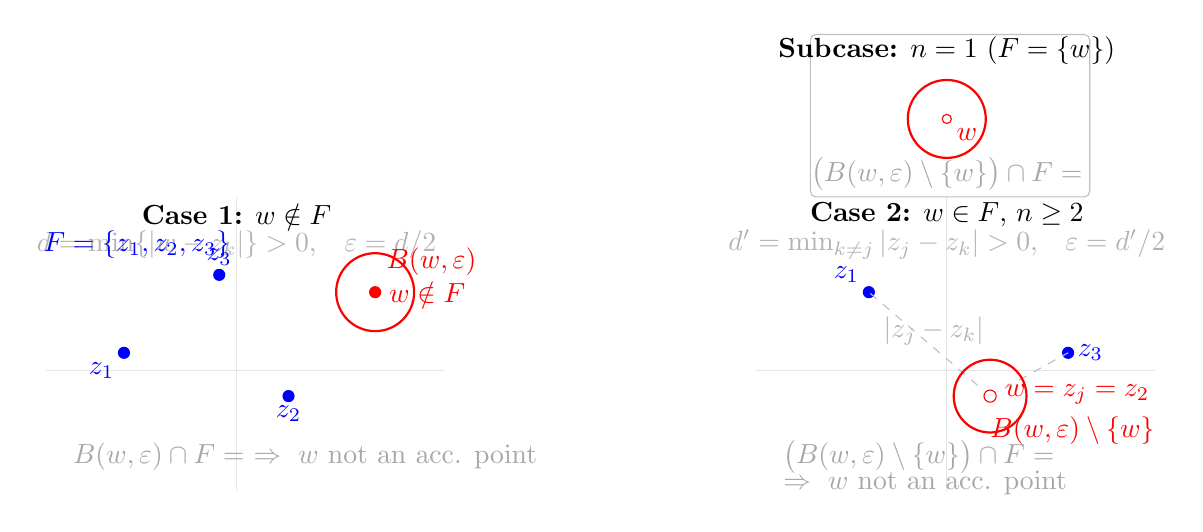
\begin{tikzpicture}[scale=1.1]
	
	% ================== Case 1: w not in F ==================
	\begin{scope}
		% axes (faint)
		\draw[gray!20] (-2.2,0) -- (2.4,0);
		\draw[gray!20] (0,-1.4) -- (0,2.0);
		
		\node[align=left] at (0,1.8) {\textbf{Case 1:} $w\notin F$};
		\node[align=left,gray!60] at (0,1.45) {$d=\min\{|w-z_k|\}>0$,\quad $\varepsilon=d/2$};
		
		% finite set F = {z1,z2,z3}
		\fill[blue] (-1.3,0.2) circle (2pt) node[below left] {$z_1$};
		\fill[blue] (0.6,-0.3)  circle (2pt) node[below] {$z_2$};
		\fill[blue] (-0.2,1.1)  circle (2pt) node[above] {$z_3$};
		\node[blue] at (-1.15,1.45) {$F=\{z_1,z_2,z_3\}$};
		
		% w not in F and its epsilon-ball
		\fill[red] (1.6,0.9) circle (2pt);
		\node[red,anchor=west] at (1.65,0.9) {$w\notin F$};
		
		% choose a ball around w that avoids F (epsilon = d/2 schematic)
		\draw[red,thick] (1.6,0.9) circle (0.45);
		\node[red] at (2.25,1.25) {$B(w,\varepsilon)$};
		
		% emphasize empty intersection
		\node[gray!70,anchor=west] at (-2.0,-1.0)
		{$B(w,\varepsilon)\cap F=\varnothing\ \Rightarrow\ \text{$w$ not an acc. point}$};
	\end{scope}
	
	% =============== Case 2: w in F, n >= 2 =================
	\begin{scope}[xshift=8.2cm]
		% axes (faint)
		\draw[gray!20] (-2.2,0) -- (2.4,0);
		\draw[gray!20] (0,-1.4) -- (0,2.0);
		
		\node[align=left] at (0,1.8) {\textbf{Case 2:} $w\in F$,\ $n\ge2$};
		\node[align=left,gray!60] at (0,1.45) {$d'=\min_{k\neq j}|z_j-z_k|>0$,\quad $\varepsilon=d'/2$};
		
		% finite set F = {z1=z_j, z2, z3}
		\fill[blue] (-0.9,0.9) circle (2pt) node[above left] {$z_1$};
		\fill[blue] (1.4,0.2)  circle (2pt) node[right] {$z_3$};
		
		% w = z2 (the point we're testing)
		\fill[red] (0.5,-0.3) circle (2pt);
		\node[red,anchor=west] at (0.56,-0.28) {$w=z_j=z_2$};
		
		% distances from w to neighbors (guides)
		\draw[gray!50,dashed] (0.5,-0.3) -- (-0.9,0.9);
		\draw[gray!50,dashed] (0.5,-0.3) -- (1.4,0.2);
		\node[gray!60] at (-0.15,0.45) {$|z_j-z_k|$};
		
		% punctured ball B(w, eps)\{w} with eps = d'/2 (schematic radius)
	\draw[red,thick] (0.5,-0.3) circle (0.42);
	% open/white dot to stress "punctured"
	\fill[white] (0.5,-0.3) circle (2.6pt);
	\draw[red] (0.5,-0.3) circle (2pt);
	\node[red] at (1.45,-0.7) {$B(w,\varepsilon)\setminus\{w\}$};
	
	% emphasize empty intersection with F\{w}
\node[gray!70,anchor=west] at (-2.0,-1.0)
{$\bigl(B(w,\varepsilon)\setminus\{w\}\bigr)\cap F=\varnothing$};
\node[gray!70,anchor=west] at (-2.0,-1.3)
{$\Rightarrow\ \text{$w$ not an acc. point}$};
\end{scope}

% =============== Inset: Case 2 with n=1 =================
\begin{scope}[xshift=8.2cm,yshift=2.9cm,scale=0.75]
% small box
\draw[gray!50,rounded corners=2pt] (-2.1,-1.2) rectangle (2.2,1.3);
\node at (0,1.05) {\textbf{Subcase:} $n=1$ ($F=\{w\}$)};

% w and its punctured ball
\fill[red] (0,0) circle (2pt) node[below right] {$w$};
\draw[red,thick] (0,0) circle (0.6);
\fill[white] (0,0) circle (2.6pt);
\draw[red] (0,0) circle (2pt);

\node[gray!70] at (0,-0.85)
{$\bigl(B(w,\varepsilon)\setminus\{w\}\bigr)\cap F=\varnothing$};
\end{scope}

\end{tikzpicture}



%\vspace{1em}
%\noindent\textbf{Source.} Adapted from the provided lecture note \emph{Complex Variables and Applications — Chapter 1: Complex Numbers}. :contentReference[oaicite:0]{index=0}


\newpage
\section{Analytic Functions}
\subsection{Functions of a Complex Variable}

\begin{definition}[Function and domain]
	Let $S\subset\C$. A \emph{function} $f$ on $S$ assigns to each $z\in S$ a complex number $w=f(z)$. The set $S$ is the \emph{domain} (domain of definition) of $f$. As real functions, we write $f(z)=u(x,y)+iv(x,y)$ for $z=x+iy$; in polar form, $f(z)=u(r,\theta)+iv(r,\theta)$. \end{definition}

\begin{definition}[Polynomials and rational functions]
	If $n\in\mathbb{Z}_{\ge0}$ and $a_0,\dots,a_n\in\C$ with $a_n\neq0$, the polynomial
	\[
	P(z)=a_0+a_1z+\cdots+a_n z^n
	\]
	has degree $n$. A \emph{rational function} is $P(z)/Q(z)$, defined where $Q(z)\neq0$.
\end{definition}

\begin{example}[Single-valued choice of a multiple-valued expression]
	For $z\neq0$ with $z=re^{i\theta}$ ($-\pi<\theta\le\pi$), the square root has two values $z^{1/2}=\pm\sqrt{r}\,e^{i\theta/2}$. Selecting the ``$+$'' value defines a single-valued branch on $\C^\times$; setting $f(0)=0$ extends it to $z=0$ (not analytic there). 
\end{example}

\subsection{Mappings}

\begin{definition}[Mapping, image, range, inverse image]
	Viewing $f$ as a mapping $f:S\to\C$, the \emph{image} of $z$ is $w=f(z)$; the image of $T\subset S$ is $f(T)$; the \emph{range} is $f(S)$. The \emph{inverse image} of $w_0$ is $\{z\in S:f(z)=w_0\}$.
\end{definition}

\begin{observation}[Basic geometric actions]
	\begin{itemize}[leftmargin=1.5em]
		\item $w=z+1$ translates one unit to the right.
		\item $w=iz=re^{i(\theta+\pi/2)}$ rotates by $\pi/2$ counterclockwise.
		\item $w=\bar z=x-iy$ reflects across the real axis.
	\end{itemize}
\end{observation}

\begin{example}[$w=z^2$ as a mapping]
	With $z=x+iy$, we have $w=u+iv$ where $u=x^2-y^2$, $v=2xy$. The first quadrant region $\{x\ge0,\,y\ge0,\,xy\le1\}$ maps onto the horizontal strip $\{0\le v\le2\}$.
\end{example}

\subsubsection*{Mapping by the exponential}
If $w=e^z=e^{x+iy}=e^x(\cos y+i\sin y)=\rho e^{i\theta}$, then $\rho=e^x$ and $\theta=y$. Thus vertical lines $\{x=\text{const}\}$ map to circles $\{|w|=\text{const}\}$ and horizontal lines $\{y=\text{const}\}$ map to rays $\{\arg w=\text{const}\}$.

\subsection{Limits and Related Theorems}

\begin{definition}[Limit]
	Let $f$ be defined on a deleted neighborhood of $z_0$. We say $\displaystyle\lim_{z\to z_0}f(z)=w_0$ if for each $\varepsilon>0$ there exists $\delta>0$ such that $|f(z)-w_0|<\varepsilon$ whenever $0<|z-z_0|<\delta$.
\end{definition}

\begin{theorem}[Uniqueness of limits]
	If the limit $\lim_{z\to z_0} f(z)$ exists, it is unique.\end{theorem}

\begin{example}
	For $f(z)=\tfrac{i}{2}z$ on $|z|<1$, $\lim_{z\to1}f(z)=\tfrac{i}{2}$. For $f(z)=\bar z/z$, $\lim_{z\to0}f(z)$ does \emph{not} exist: approaching along the real axis gives $1$, along the imaginary axis gives $-1$.
\end{example}

\begin{theorem}[Limit laws]
	If $\lim_{z\to z_0} f(z)=f_0$ and $\lim_{z\to z_0} g(z)=g_0$, then
	\[
	\lim_{z\to z_0}\big(f+g\big)=f_0+g_0,\quad
	\lim_{z\to z_0} f\,g=f_0g_0,\quad
	\lim_{z\to z_0}\frac{f}{g}=\frac{f_0}{g_0}\ (g_0\neq0).
	\]
	In particular, polynomials are continuous: $\lim_{z\to z_0}P(z)=P(z_0)$.
\end{theorem}

\subsubsection{Limits involving $\infty$}
Neighborhoods of $\infty$ are exteriors of large disks. One has
\[
\lim_{z\to z_0} f(z)=\infty \iff \lim_{z\to z_0}\frac{1}{f(z)}=0,\qquad
\lim_{z\to\infty} f(z)=w_0 \iff \lim_{z\to0} f\!\left(\tfrac1z\right)=w_0,
\]
and $\lim_{z\to\infty} f(z)=\infty \iff \lim_{z\to0} \frac{1}{f(1/z)}=0$.

\subsection{Continuity}

\begin{definition}[Continuity]
	$f$ is continuous at $z_0$ if $\lim_{z\to z_0}f(z)=f(z_0)$. It is continuous on a region $R$ if continuous at each $z_0\in R$.
\end{definition}

\begin{theorem}[Basic properties]
	Composition of continuous functions is continuous. If $f$ is continuous and $f(z_0)\neq0$, then $f$ is nonzero on some neighborhood of $z_0$. If $f=u+iv$, then $f$ is continuous at $z_0$ iff $u$ and $v$ are continuous there. If $R$ is closed and bounded and $f$ continuous on $R$, then $|f|$ attains a maximum on $R$ (boundedness).
\end{theorem}

\subsection{Derivatives}

\begin{definition}[Complex derivative]
	If $f$ is defined on a neighborhood of $z_0$, the derivative at $z_0$ is
	\[
	f'(z_0)=\lim_{z\to z_0}\frac{f(z)-f(z_0)}{z-z_0}
	=\lim_{\Delta z\to0}\frac{\Delta w}{\Delta z},\quad \Delta w=f(z_0+\Delta z)-f(z_0),
	\]
	when the limit exists.
\end{definition}

\begin{theorem}[Consequences]
	If $f'(z_0)$ exists then $f$ is continuous at $z_0$. Moreover,
	\[
	\frac{d}{dz}c=0,\qquad \frac{d}{dz}z=1,\qquad \frac{d}{dz}[c f]=c f',\qquad
	\frac{d}{dz}z^n=n z^{n-1}\ (n\in\mathbb{Z},\ z\neq0\text{ if }n<0),
	\]
	and the sum/product/quotient rules and chain rule hold exactly as in calculus.
\end{theorem}

\begin{example}
	$f(z)=z^2\Rightarrow f'(z)=2z$. The function $f(z)=\bar z$ has no complex derivative anywhere. The function $f(z)=|z|^2$ has derivative only at $z=0$ (value $0$).
\end{example}

\subsection{Cauchy--Riemann Equations}

Let $f=u+iv$ with $u,v$ real-valued.

\begin{theorem}[Cauchy--Riemann (CR) equations]
	If $f'(z_0)$ exists then the first partials of $u,v$ exist at $(x_0,y_0)$ and satisfy
	\[
	u_x(x_0,y_0)=v_y(x_0,y_0),\qquad u_y(x_0,y_0)=-v_x(x_0,y_0),
	\]
	and $f'(z_0)=u_x(x_0,y_0)+i\,v_x(x_0,y_0)$.
\end{theorem}

\begin{theorem}[Sufficient conditions]
	If $u_x,u_y,v_x,v_y$ exist in a neighborhood of $z_0$, are continuous at $z_0$, and satisfy the CR equations at $z_0$, then $f'(z_0)$ exists and equals $u_x+i v_x$.
\end{theorem}

\begin{example}
	$f(z)=z^2=x^2-y^2+i\,2xy$ satisfies CR everywhere and $f'(z)=2z$. For $f(z)=|z|^2=x^2+y^2$, the CR equations force $(x,y)=(0,0)$; hence $f'$ exists only at $0$. For $f(z)=e^z=e^x(\cos y+i\sin y)$ we have $f'(z)=e^z$ for all $z$.
\end{example}

\subsubsection*{CR equations in polar coordinates}
If $f=u(r,\theta)+iv(r,\theta)$ near $z_0=r_0e^{i\theta_0}\neq0$, the polar CR system is
\[
u_r=\frac1r v_\theta,\qquad v_r=-\frac1r u_\theta,
\]
and $f'(z_0)=e^{-i\theta_0}\big(u_r(r_0,\theta_0)+i\,v_r(r_0,\theta_0)\big)$.

\subsection{Analytic Functions}

\begin{definition}[Analytic/entire/singularity]
	$f$ is \emph{analytic} at $z_0$ if it has a derivative at every point of some neighborhood of $z_0$. If analytic at every point of $\C$, $f$ is \emph{entire}. If $f$ fails to be analytic at $z_0$ but is analytic arbitrarily close to $z_0$, then $z_0$ is a \emph{singular point} (singularity) of $f$.
\end{definition}

\begin{theorem}[Algebra and composition]
	Sums and products of analytic functions are analytic; a quotient $f/g$ is analytic where $g\neq0$. If $f$ is analytic in $D$ and $g$ is analytic on $f(D)$, then $g\circ f$ is analytic in $D$ with $(g\circ f)'=(g'\circ f)\,f'$.
\end{theorem}

\begin{theorem}[Zero derivative]
	If $f'(z)=0$ for all $z$ in a domain $D$, then $f$ is constant on $D$.
\end{theorem}

\begin{example}
	\[
	f(z)=\frac{z^3+4}{(z^2-3)(z^2+1)}
	\]
	is analytic on $\C\setminus\{\pm\sqrt{3},\,\pm i\}$. Also $f(z)=\cosh x\cos y+i\sinh x\sin y$ is entire since CR holds everywhere.
\end{example}

\begin{theorem}[Conjugate tests]
	If $f$ and $\bar f$ are both analytic in $D$, then $f$ is constant in $D$. If $f$ is analytic in $D$ and $|f|$ is constant, then $f$ is constant.
\end{theorem}

\subsection{Harmonic Functions}

\begin{definition}[Harmonicity]
	A real function $h(x,y)$ is \emph{harmonic} on a domain if it has continuous second partials and satisfies Laplace's equation
	\[
	\Delta h=h_{xx}+h_{yy}=0.
	\]
\end{definition}

\begin{theorem}[Harmonic components]
	If $f=u+iv$ is analytic in $D$, then $u$ and $v$ are harmonic in $D$. Conversely, if $u$ and $v$ are harmonic and satisfy the CR equations in $D$, then $f=u+iv$ is analytic in $D$; $v$ is then a \emph{harmonic conjugate} of $u$.
\end{theorem}

\begin{example}
	$f(z)=\dfrac{i}{z^2}$ is analytic on $\C\setminus\{0\}$; writing it as
	\[
	\frac{i}{z^2}=\frac{2xy+i(x^2-y^2)}{(x^2+y^2)^2}=u+iv,
	\]
	both $u$ and $v$ are harmonic away from the origin. For $u(x,y)=y^3-3x^2y$, a harmonic conjugate is $v(x,y)=-3xy^2+x^3+C$.
\end{example}

\subsubsection*{Uniqueness and reflection}
\begin{lemma}[Identity lemma]
	If $f$ is analytic in $D$ and vanishes on a set with a limit point in $D$ (e.g.\ a subdomain or line segment), then $f\equiv0$ in $D$.
\end{lemma}

\begin{theorem}[Uniqueness from values]
	An analytic function in $D$ is uniquely determined in $D$ by its values on any subdomain or line segment contained in $D$.
\end{theorem}

\begin{theorem}[Reflection principle (real axis)]
	Let $D$ contain a symmetric neighborhood of a real segment. Then $f(\bar z)=\overline{f(z)}$ in $D$ iff $f(x)\in\R$ for all $x$ on that segment.
\end{theorem}

\newpage
\section*{Exercises}
\begin{enumerate}[\bfseries 1.]
\item Show that the following limit does not exitst \[
\lim_{z\to0}\Big(\frac{\bar z}{z}\Big)^2
\] Do this by letting nonzero points $z=(x,0)$ and $z=(x,x)$ approach the origin. (Note that it is not sufficient to simply consider points $z=(x,0)$ and $z=(0,y)$.)
\begin{proof}[\Sol]
Let $z=x+iy\in\C$ with $x,y\in\mathbb{R}$. Then \[
\left(\frac{\overline{z}}{z}\right)^{\!2}
=\left(\frac{x-iy}{x+iy}\right)^{\!2}.
\] If $z=re^{i\theta}$ with $r>0$, then $\bar z/z=e^{-2i\theta}$, so $|(\bar z/z)^2|=|e^{-4i\theta}|=1$.
\begin{center}
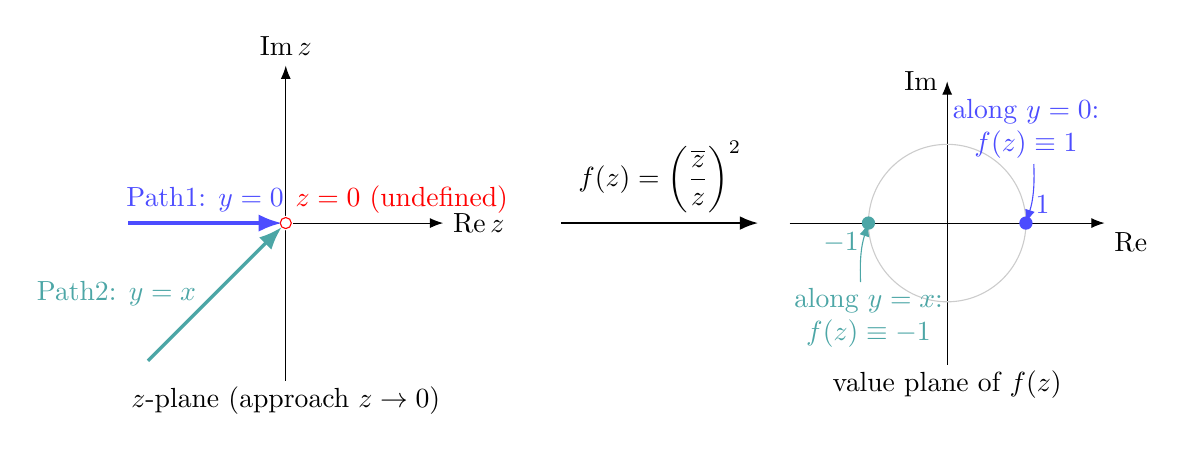
\begin{tikzpicture}[>=Latex,scale=1]
% =============== z-plane (paths to the origin) ===============
\begin{scope}
	% axes
	\draw[->] (-2.0,0) -- (2.0,0) node[right] {$\Re z$};
	\draw[->] (0,-2.0) -- (0,2.0) node[above] {$\Im z$};
	\node at (0,-2.25) {$z$-plane (approach $z\to 0$)};
	
	% origin as a hole (z=0 excluded)
	\fill[white] (0,0) circle (2.6pt);
	\draw[red] (0,0) circle (2pt) node[above right] {$z=0$ (undefined)};
	
	% Path 1: real axis y=0 (blue)
	\draw[blue!70,very thick,->] (-2,0) -- (-0.05,0) node[midway, above] {Path1: $y=0$};
	
	% Path 2: diagonal y=x (teal)
	\draw[teal!70,very thick,->] (-1.75,-1.75) -- (-0.05,-0.05) node[midway, xshift=-1.25cm] {Path2: $y=x$};
\end{scope}
% =============== mapping arrow ===============
\draw[->,thick] (3.5,0) -- (6,0)
node[midway,above] {$f(z)=\left(\dfrac{\overline z}{z}\right)^2$};
% =============== value plane (outputs) ===============
\begin{scope}[xshift=8.4cm]
	% axes
	\draw[->] (-2,0) -- (2,0) node[below right] {$\Re$};
	\draw[->] (0,-1.8) -- (0,1.8) node[left] {$\Im$};
	\node at (0,-2.05) {value plane of $f(z)$};
	
	% unit circle (context): |(\bar z/z)^2| = 1 for z≠0
	\draw[gray!40] (0,0) circle (1);
	
	% images of the two paths (constants 1 and -1)
	% Path 1 (y=0) -> 1
	\fill[blue!70] (1,0) circle (2.4pt) node[above right] {$1$};
	\draw[blue!70,->] (1.1,.75) to[bend left=10] (1,0);
	\node[blue!70,align=center] at (1,1.2)
	{along $y=0$:\\ $f(z)\equiv 1$};
	
	% Path 2 (y=x) -> -1
	\fill[teal!70] (-1,0) circle (2.4pt) node[below left] {$-1$};
	\draw[teal!70,->] (-1.1,-0.75) to[bend left=10] (-1,0);
	\node[teal!70,align=center] at (-1,-1.2)
	{along $y=x$:\\ $f(z)\equiv -1$};
	
%	% conclusion box
%	\node[draw,rounded corners=2pt,align=left,anchor=north] at (0,-1.25)
%	{$\displaystyle \lim_{z\to 0}\left(\frac{\overline z}{z}\right)^2\ \text{does not exist},$\\
%		since the limits along $y=0$ and $y=x$ differ.};
\end{scope}
\end{tikzpicture}
\end{center}
\medskip
\noindent\textbf{(1) Path 1: approach along the real axis $y=0$}

Let $z=x+0i=x$ with $x\in\mathbb{R}\setminus\{0\}$ and $x\to 0$. Then $
\displaystyle\left(\frac{\overline{z}}{z}\right)^2
=\left(\frac{x}{x}\right)^2
=1$.

\medskip
\noindent\textbf{(2) Path 2: approach along the diagonal $y=x$}

Let $z=x+ix=(1+i)x$ with $x\in\mathbb{R}\setminus\{0\}$ and $x\to 0$. Then
\[
\frac{\overline{z}}{z}
=\frac{\overline{(1+i)x}}{(1+i)x}
=\frac{(1-i)\,x}{(1+i)\,x}
=\frac{1-i}{1+i}
=\frac{(1-i)^2}{(1+i)(1-i)}
=\frac{1-2i+i^2}{1- i^2}
=\frac{1-2i-1}{2}
=\frac{-2i}{2}
=-i.
\]
Hence
\[
\left(\frac{\overline{z}}{z}\right)^2
=(-i)^2
=-1.
\] 

\medskip
\noindent\textbf{(3) Conclusion}

Since the limits along these two paths are different (namely $1$ and $-1$), the limit cannot exist.
\end{proof}
%	\item[X] Compute $\displaystyle \lim_{z\to\infty}\frac{4z^2}{(z-1)^2}$, $\ \lim_{z\to1}\frac{1}{(z-1)^3}$, and $\ \lim_{z\to\infty}\frac{z^2+1}{z-1}$.
%	\item[X] Suppose $f(z_0)=g(z_0)=0$ with $g'(z_0)\neq0$ and both derivatives exist. Prove
%	\[
%	\lim_{z\to z_0}\frac{f(z)}{g(z)}=\frac{f'(z_0)}{g'(z_0)}.
%	\]
\item Let \[
f(z)=\begin{cases} \bar z^2/z,& z\neq0,\\ 0,& z=0.\end{cases}
\] Show that if $z=0$, then $\Delta w/\Delta z=1$ at eatch nonzero point on the real and imaginary axes in the $\Delta z$, or $\Delta x\Delta y$, plane. Then show that $\Delta w/\Delta z=-1$ at each nonzero point $(\Delta x, \Delta y)$ on the line $\Delta y=\Delta x$ in that plane. Conclude from these observations that $f'(0)$ does not exist. Note that to obtain this result, it is not sufficient to consider only horizontal and vertical approaches to the origin in the $\Delta z$ plane.
\begin{proof}
Let $\frac{\Delta w}{\Delta z}
=\frac{f(\Delta z)-f(0)}{\Delta z}
\quad(\Delta z\neq 0)$. Since $f(0)=0$, for $\Delta z\neq0$, $\displaystyle
\frac{\Delta w}{\Delta z}
=\frac{f(\Delta z)}{\Delta z}
=\frac{\overline{\Delta z}^{\,2}}{(\Delta z)^2}$.

\medskip
\noindent\textbf{(1) Real and imaginary axes.}
\begin{itemize}
	\item Real axis: $\Delta z=x$ with $x\in\mathbb{R}\setminus\{0\}$, $\displaystyle
	\frac{\Delta w}{\Delta z}=\frac{\overline{x}^{\,2}}{x^2}=\frac{x^2}{x^2}=1$.
	\begin{center}
	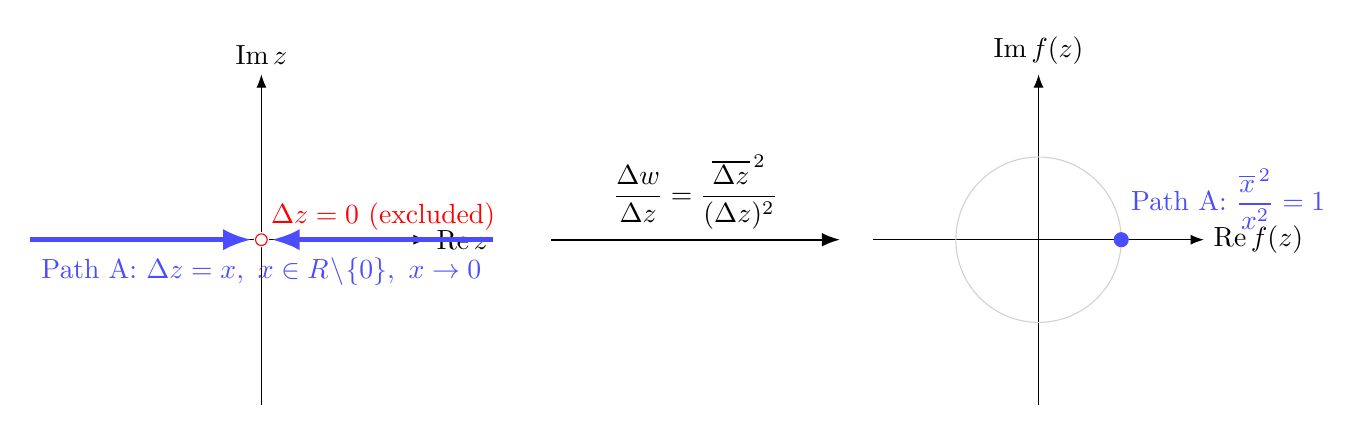
\begin{tikzpicture}[>=Latex,scale=1.05]	
		%================ z-plane: explicit paths =================
		\begin{scope}
			% axes
			\draw[->] (-2,0) -- (2,0) node[right] {$\Re z$};
			\draw[->] (0,-2) -- (0,2) node[above] {$\Im z$};
			% hole at the origin (Delta z = 0 excluded)
			\fill[white] (0,0) circle (2.6pt);
			\draw[red] (0,0) circle (2pt) node[above right] {$\Delta z=0$ (excluded)};
			% Path A: real axis, Δz = x, x→0, x≠0
			\draw[line width=1.6pt,blue!70,->] (-2.8,0) -- (-0.12,0);
			\draw[line width=1.6pt,blue!70,->] ( 2.8,0) -- ( 0.12,0);
			\node[blue!70,anchor=north] at (0,-0.10)
			{$\displaystyle \text{Path A: }\Delta z=x,\ x\in\mathbb R\!\setminus\!\{0\},\ x\to 0$};
		\end{scope}
		%================ mapping arrow =================
		\draw[->,thick] (3.5,0) -- (7,0)
		node[midway,above] {$\displaystyle \frac{\Delta w}{\Delta z}=\frac{\overline{\Delta z}^{\,2}}{(\Delta z)^2}$};
		%================ value plane: constant images =================
		\begin{scope}[xshift=9.4cm]
			% axes
			\draw[->] (-2,0) -- (2,0) node[right] {$\Re f(z)$};
			\draw[->] (0,-2) -- (0,2) node[above] {$\Im f(z)$};
			%	\node at (0,-2.55) {$f(z)$-plane of $\Delta w/\Delta z$};
			% unit circle for context (|Δw/Δz|=1 for Δz≠0)
			\draw[gray!35] (0,0) circle (1);
			% Image of Path A (real axis): constant 1
			\fill[blue!70] (1,0) circle (2.6pt) node[above right] {$\displaystyle \text{Path A: } \frac{\overline{x}^{\,2}}{x^2}=1$};
		\end{scope}
	\end{tikzpicture}
	\end{center}
	\item Imaginary axis: $\Delta z=iy$ with $y\in\mathbb{R}\setminus\{0\}$, $\displaystyle
	\frac{\Delta w}{\Delta z}
	=\frac{\overline{iy}^{\,2}}{(iy)^2}
	=\frac{(-iy)^2}{(iy)^2}
	=\frac{-y^2}{-y^2}=1$.
	\begin{center}
	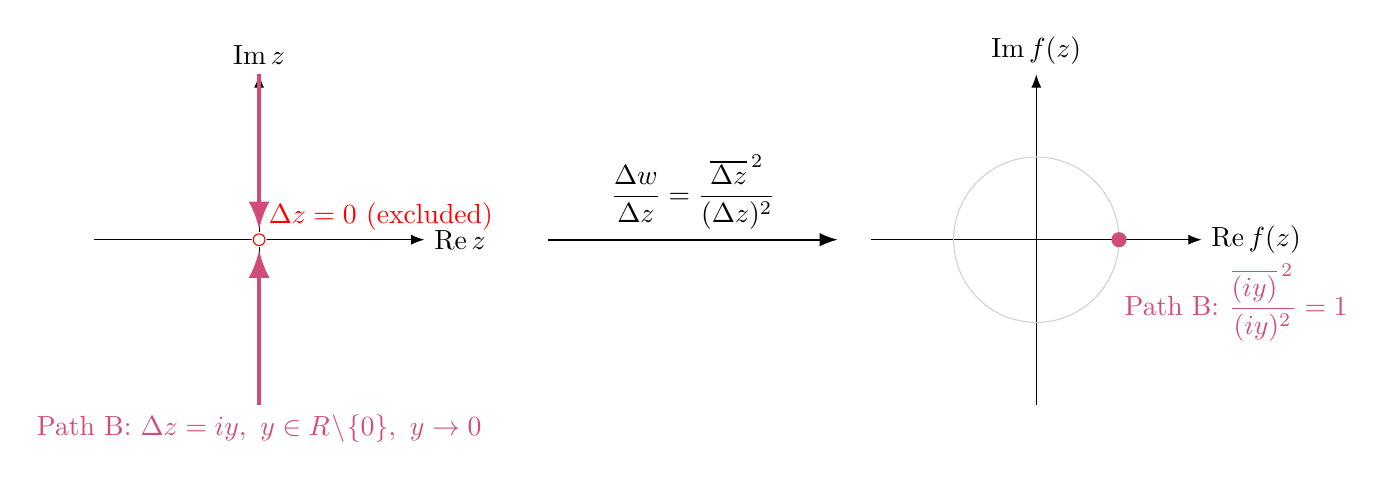
\begin{tikzpicture}[>=Latex,scale=1.05]	
		%================ z-plane: explicit paths =================
		\begin{scope}
			% axes
			\draw[->] (-2,0) -- (2,0) node[right] {$\Re z$};
			\draw[->] (0,-2) -- (0,2) node[above] {$\Im z$};
			% hole at the origin (Delta z = 0 excluded)
			\fill[white] (0,0) circle (2.6pt);
			\draw[red] (0,0) circle (2pt) node[above right] {$\Delta z=0$ (excluded)};
			% Path B: imaginary axis, Δz = iy, y→0, y≠0
			\draw[line width=1.6pt,purple!70,->] (0,-2.0) -- (0,-0.12);
			\draw[line width=1.6pt,purple!70,->] (0, 2.0) -- (0, 0.12);
			\node[purple!70,anchor=north] at (0,-2)
			{$\displaystyle \text{Path B: }\Delta z=iy,\ y\in\mathbb R\!\setminus\!\{0\},\ y\to 0$};
		\end{scope}
		%================ mapping arrow =================
		\draw[->,thick] (3.5,0) -- (7,0)
		node[midway,above] {$\displaystyle \frac{\Delta w}{\Delta z}=\frac{\overline{\Delta z}^{\,2}}{(\Delta z)^2}$};
		%================ value plane: constant images =================
		\begin{scope}[xshift=9.4cm]
			% axes
			\draw[->] (-2,0) -- (2,0) node[right] {$\Re f(z)$};
			\draw[->] (0,-2) -- (0,2) node[above] {$\Im f(z)$};
			%	\node at (0,-2.55) {$f(z)$-plane of $\Delta w/\Delta z$};
			% unit circle for context (|Δw/Δz|=1 for Δz≠0)
			\draw[gray!35] (0,0) circle (1);
			% Image of Path B (imag axis): constant 1
			\fill[purple!70] (1,0) circle (2.6pt);
			\node[purple!70,anchor=north west] at (0.95,-0.18)
			{$\displaystyle \text{Path B: } \frac{\overline{(iy)}^{\,2}}{(iy)^2}=1$};
		\end{scope}
	\end{tikzpicture}
	\end{center}
\end{itemize}

\noindent\textbf{(2) Line $\Delta y=\Delta x$.}
Let $\Delta z=(1+i)x$ with $x\in\mathbb{R}\setminus\{0\}$. Then
\[
\frac{\Delta w}{\Delta z}
=\frac{\overline{(1+i)x}^{\,2}}{((1+i)x)^2}
=\frac{((1-i)x)^2}{((1+i)x)^2}
=\frac{(1-i)^2}{(1+i)^2}
=\frac{-2i}{2i}=-1.
\]
\begin{center}
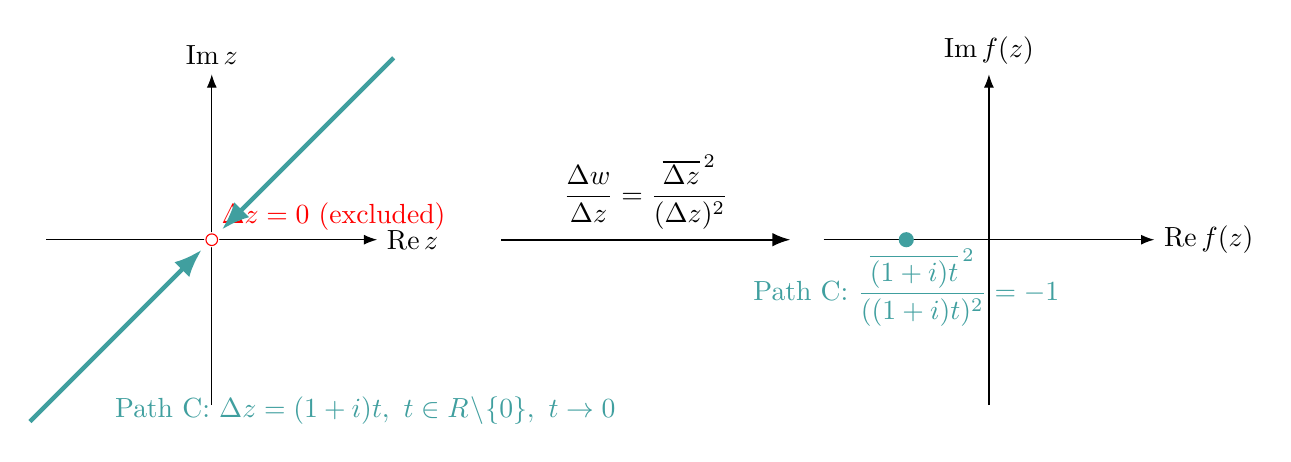
\begin{tikzpicture}[>=Latex,scale=1.05]	
%================ z-plane: explicit paths =================
\begin{scope}
	% axes
	\draw[->] (-2,0) -- (2,0) node[right] {$\Re z$};
	\draw[->] (0,-2) -- (0,2) node[above] {$\Im z$};
	%	\node at (0,-2.55) {$z$-plane (approach $\Delta z\to 0$)$\,$};	
	% hole at the origin (Delta z = 0 excluded)
	\fill[white] (0,0) circle (2.6pt);
	\draw[red] (0,0) circle (2pt) node[above right] {$\Delta z=0$ (excluded)};
	% Path C: diagonal Δy=Δx, i.e., Δz = (1+i)t, t→0, t≠0
	\draw[line width=1.6pt,teal!75,->] (-2.2,-2.2) -- (-0.12,-0.12);
	\draw[line width=1.6pt,teal!75,->] ( 2.2, 2.2) -- ( 0.12, 0.12);
	\node[teal!75,anchor=south east] at (5,-2.35)
	{$\displaystyle \text{Path C: }\Delta z=(1+i)t,\ t\in\mathbb R\!\setminus\!\{0\},\ t\to 0$};
\end{scope}
%================ mapping arrow =================
\draw[->,thick] (3.5,0) -- (7,0)
node[midway,above] {$\displaystyle 
	\frac{\Delta w}{\Delta z}=\frac{\overline{\Delta z}^{\,2}}{(\Delta z)^2}
	%	\displaystyle \,f(z)=\begin{cases}
		%		\overline z^{\,2}/z &\text{if}\; z\neq 0\\
		%		0 &\text{if}\; z=0
		%	\end{cases}
	$};
%================ value plane: constant images =================
\begin{scope}[xshift=9.4cm]
	% axes
	\draw[->] (-2,0) -- (2,0) node[right] {$\Re f(z)$};
	\draw[->] (0,-2) -- (0,2) node[above] {$\Im f(z)$};
	%	\node at (0,-2.55) {$f(z)$-plane of $\Delta w/\Delta z$};
	% Image of Path C (diagonal): constant -1
	\fill[teal!75] (-1,0) circle (2.6pt) node[below] {$\displaystyle \text{Path C: } \frac{\overline{(1+i)t}^{\,2}}{((1+i)t)^2}=-1$};
\end{scope}
\end{tikzpicture}
\end{center}
\medskip
\noindent\textbf{(3) Conclusion.}
Since the difference quotient equals $1$ along the axes but $-1$ along the line $\Delta y=\Delta x$, the limit
\[
\lim_{\Delta z\to 0}\frac{f(\Delta z)-f(0)}{\Delta z}
\]
depends on the path and therefore does not exist. Consequently, $f'(0)$ does not exist.
\end{proof}	
\newpage
\item Let \[
f(z)=\bar z,\quad f(z)=2x+ixy^2,\quad f(z)=e^{\bar z}
\] Then show that $f'(z)$ does not exists at any point.
\begin{proof}[\Sol]
Let \(z=x+iy\) and \(f(z)=u+iv\) with $x,y,u,v\in\R$. The Cauchy--Riemann equations \[
u_x=v_y,\qquad u_y=-\,v_x
\]
are necessary and sufficient for complex differentiability.

\medskip
\noindent\textbf{(1) \(f_1(z)=\overline z=\overline{x+iy}=x-iy\).}

Here \(u(x,y)=x,\ v(x,y)=-y\). Thus \[
u_x=1,\quad u_y=0,\quad v_x=0,\quad v_y=-1.
\]
The CR require \(u_x=v_y\), i.e.\ \(1=-1\), which is impossible. Hence \(f_1'\) does not exist anywhere.

\medskip
\noindent\textbf{(2) \(f_2(z)=2x+i\,x y^{2}\).}

Here \(u(x,y)=2x,\ v(x,y)=x y^{2}\). Thus
\[
u_x=2,\quad u_y=0,\quad v_x=y^{2},\quad v_y=2xy.
\]
The CR demand \[
\begin{cases} u_x=v_y\\ u_y=-v_x \end{cases}\implies
\begin{cases} 2=2xy\\ 0=y^2 \end{cases}\implies
\begin{cases} xy=1\\ y=0 \end{cases}.
\] These cannot hold simultaneously for any \(x\). Hence CR fail at every point, so \(f_2'\) exists nowhere.

\medskip
\noindent\textbf{(3) \(f_3(z)=e^{\overline z}\).}

Let \(\overline z=x-iy\). Then $f_3(x,y)=e^{x-iy}=e^{x}(\cos y-i\sin y)$, so \[
u(x,y)=e^{x}\cos y,\qquad v(x,y)=-\,e^{x}\sin y.
\] Compute \[
u_x=e^{x}\cos y,\quad u_y=-e^{x}\sin y,\quad
v_x=-e^{x}\sin y,\quad v_y=-e^{x}\cos y.
\] The CR give \[
\begin{cases} u_x=v_y\\ u_y=-v_x \end{cases}\implies
\begin{cases} e^x\cos y=-e^x\cos y\\ -e^x\sin y=+e^x\sin y \end{cases}\implies
\begin{cases} \cos y = 0\\ \sin y=0 \end{cases}.
\] These cannot hold simultaneously for any \(y\). Hence CR fail everywhere and \(f_3'\) exists nowhere.
\end{proof}
\item Let $f(z)=u(x,y)+i v(x,y)$ be given by \[
f(z)=\begin{cases}
	\bar z^2/z &: z\neq 0 \\
	0 &: z=0.
\end{cases}
\] Verify that the Cauchy--Riemann equations $u_x=v_y$ and $u_y=-v_x$ are satisfied at the origin $z=(0,0)$.
\begin{proof}
Write $z=x+iy$ and define
\[
f(z)=
\begin{cases}
	\dfrac{\overline z^{\,2}}{z}, & (x,y)\neq(0,0),\\[4pt]
	0, & (x,y)=(0,0).
\end{cases}
\]
Let $f=u+iv$. We compute the first-order partials of $u,v$ at $(0,0)$ by restricting to the
coordinate axes.

\medskip
\noindent\textbf{Along the $x$-axis ($y=0$):} For $x\neq0$,
\[
f(x,0)=\frac{\overline{x}^{\,2}}{x}=x,
\]
hence $u(x,0)=x$ and $v(x,0)=0$. Therefore
\[
u_x(0,0)=\lim_{h\to0}\frac{u(h,0)-u(0,0)}{h}
=\lim_{h\to0}\frac{h-0}{h}=1,
\quad
v_x(0,0)=\lim_{h\to0}\frac{v(h,0)-v(0,0)}{h}
=\lim_{h\to0}\frac{0-0}{h}=0.
\]

\medskip
\noindent\textbf{Along the $y$-axis ($x=0$):} For $y\neq0$,
\[
f(0,y)=\frac{\overline{iy}^{\,2}}{iy}=\frac{(-iy)^2}{iy}=\frac{-y^2}{iy}=iy,
\]
so $u(0,y)=0$ and $v(0,y)=y$. Hence
\[
u_y(0,0)=\lim_{k\to0}\frac{u(0,k)-u(0,0)}{k}
=\lim_{k\to0}\frac{0-0}{k}=0,
\quad
v_y(0,0)=\lim_{k\to0}\frac{v(0,k)-v(0,0)}{k}
=\lim_{k\to0}\frac{k-0}{k}=1.
\]

\medskip
Thus at $(0,0)$ we have
\[
u_x(0,0)=1,\qquad v_y(0,0)=1,\qquad u_y(0,0)=0,\qquad v_x(0,0)=0,
\]
and consequently the Cauchy--Riemann equations
\(
u_x=v_y
\)
and
\(
u_y=-v_x
\)
hold at the origin.

\begin{remark}
	Although the Cauchy--Riemann equations hold at $(0,0)$, the complex derivative $f'(0)$ does not exist
	(since $\frac{f(\Delta z)-f(0)}{\Delta z}=\frac{\overline{\Delta z}^{\,2}}{(\Delta z)^2}$ takes different
	values along different approach directions).
\end{remark}
\end{proof}
\item Let \[
f(z)=\sin x\cosh y+i\cos x\sinh y\quad\text{and}\quad f(z)=e^{-y}(\sin x-i\cos x).
\] Then show that all $f$ are entire.
\begin{proof}[\sol]
Let \begin{align*}
f_1(z)&=\sin x\cosh y+i\cos x\sinh y\quad\text{and}\\
f_2(z)&=e^{-y}(\sin x-i\cos x).
\end{align*}
\textbf{(a) } 
Let $z = x + iy$ with $x,y \in \mathbb{R}$. Note that \[
\begin{array}{lcr}
	e^{iz}=\cos z+i\sin z && \displaystyle\cos z = \frac{e^{iz} + e^{-iz}}{2} \\
	&\longleftrightarrow& \\
	e^{-iz}=\cos z-i\sin z && \displaystyle\sin z = \frac{e^{iz} - e^{-iz}}{2i}
\end{array}
\]By definition,
\[
\sin z = \frac{e^{iz} - e^{-iz}}{2i}.
\]
Substitute $z = x + iy$:
\[
iz = i(x+iy) = ix - y, \qquad -iz = -ix + y,
\]
so
\[
e^{iz} = e^{ix-y} = e^{-y}e^{ix}, \qquad e^{-iz} = e^{-ix+y} = e^{y}e^{-ix}.
\]
Using Euler's formula $e^{ix} = \cos x + i\sin x$ and $e^{-ix} = \cos x - i\sin x$, we get
\[
e^{iz} = e^{-y}(\cos x + i\sin x), \qquad
e^{-iz} = e^{y}(\cos x - i\sin x).
\]
Then
\begin{align*}
	e^{iz} - e^{-iz}
	&= e^{-y}(\cos x + i\sin x) - e^{y}(\cos x - i\sin x) \\
	&= \cos x(e^{-y} - e^{y}) + i\sin x(e^{-y} + e^{y}).
\end{align*}
Recall the hyperbolic functions
\[
\cosh y = \frac{e^{y} + e^{-y}}{2}, \qquad
\sinh y = \frac{e^{y} - e^{-y}}{2},
\]
so that
\[
e^{-y} + e^{y} = 2\cosh y, \qquad
e^{-y} - e^{y} = -2\sinh y.
\]
Hence
\begin{align*}
	e^{iz} - e^{-iz}
	&= \cos x(-2\sinh y) + i\sin x(2\cosh y) \\
	&= 2\bigl(i\sin x\cosh y - \cos x\sinh y\bigr).
\end{align*}
Therefore
\begin{align*}
	\sin z
	&= \frac{e^{iz} - e^{-iz}}{2i}
	= \frac{2\bigl(i\sin x\cosh y - \cos x\sinh y\bigr)}{2i} \\
	&= \frac{i\sin x\cosh y}{i} - \frac{\cos x\sinh y}{i} \\
	&= \sin x\cosh y + i\cos x\sinh y,
\end{align*}
since $\dfrac{1}{i} = -i$.

Thus
\[
\boxed{\sin(x+iy) = \sin x \cosh y + i \cos x \sinh y.}
\]


Using the standard identity for the complex sine,
\[
\sin z=\sin(x+iy)=\sin x\cosh y + i\cos x\sinh y,
\]
we see immediately that $f_1(z)=\sin z$. Since $\sin z$ is an entire function (power series with infinite radius of convergence), $f_1$ is entire.

\smallskip
\textbf{(b) } Note that
\[
e^{iz}=e^{i(x+iy)}=e^{ix-y}=e^{-y}\bigl(\cos x + i\sin x\bigr).
\]
Multiplying by $-i$ gives
\[
-i\,e^{iz}=e^{-y}\bigl(\sin x - i\cos x\bigr)=f_2(z).
\]
Thus $f_2(z)=-i\,e^{iz}$. Since the exponential is entire and multiplication by a constant preserves holomorphy, $f_2$ is entire.

\smallskip
Therefore both functions are entire.
\end{proof}
	\newpage	
	\item Show that the function \[
	f(z)=\ln r+i\theta\quad (r>0,\; 0<\theta<2\pi)
	\] is analytic in the indicated domain of definition, with derivative $f'(z)=1/z$. Then show that th e composite function $g(z)=f(z^2+1)$ is analytic in the quadratic $x>0,y>0$ with derivative \[
	g'(z)=\frac{2z}{z^2+1}.
	\] (Suggestion: Observe that $\Im(z^2+1)>0$ when $x>0, y>0$)
\begin{proof}[\sol]
	Let $z=x+iy=re^{i\theta}$ with $r=\sqrt{x^2+y^2}>0$ and $0<\theta<2\pi$. Define
	\[
	f(z)=\ln r+i\theta .
	\]
	Then $f$ is analytic on the slit plane
	\begin{center}
	\begin{minipage}{.475\textwidth} \[
	\Omega:=\{\,z\in\mathbb{C}: r>0,\ 0<\theta<2\pi\,\}=\mathbb{C}\setminus[0,\infty),
	\] and $f'(z)=\frac{1}{z}\; (z\in\Omega)$.
	\end{minipage}\hfill
	\begin{minipage}{.475\textwidth}\centering
	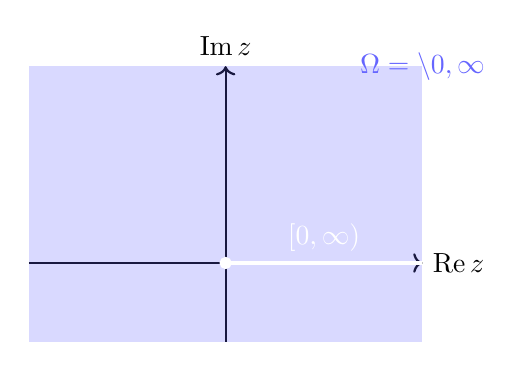
\begin{tikzpicture}
		% axes
		\draw[->, thick] (-2.5,0) -- (2.5,0) node[right] {$\Re z$};
		\draw[->, thick] (0,-1) -- (0,2.5) node[above] {$\Im z$};
		% shade domain
		\fill[blue!60, opacity=.25] (-2.5,-1) rectangle (2.5,2.5);
		\node[blue!60] at (2.5,2.5) {$\Omega=\C\setminus\intco{0,\infty}$};
		% slit: [0, +∞) on real axis
		\filldraw[white] (0,0) circle (2pt);
		\draw[white,ultra thick] (0,0) -- (2.5,0) node[midway, above] {$[0,\infty)$};
	\end{tikzpicture}
	\end{minipage}
	\end{center}
	Write $f=u+iv$ with \[
	u(x,y)=\ln r=\frac12\ln(x^2+y^2),\qquad v(x,y)=\theta=\Arg(z)\in(0,2\pi).
	\]
	On $\Omega$ the functions $u,v$ are $C^1$ and their partials are:
	\[
	u_x=\frac{x}{x^2+y^2},\quad u_y=\frac{y}{x^2+y^2},\qquad
	v_x=-\frac{y}{x^2+y^2},\quad v_y=\frac{x}{x^2+y^2}.
	\]
	Hence the Cauchy--Riemann equations hold on $\Omega$:
	\[
	u_x=v_y=\frac{x}{x^2+y^2},\qquad u_y=-v_x=\frac{y}{x^2+y^2}.
	\]
	Since these partials are continuous on $\Omega$, $f$ is analytic there. Its complex derivative is
	\[
	f'(z)=u_x+iv_x=\frac{x}{x^2+y^2}+i\!\left(-\frac{y}{x^2+y^2}\right)
	=\frac{x-iy}{x^2+y^2}=\frac{1}{x+iy}=\frac{1}{z}.
	\]
	For $g(z)=f(z^2+1)$, compute
	\begin{align*}
	z^2+1&=(x+iy)^2+1\\
	&=(x^2-y^2+2ixy) +1 \\
	&=(x^2-y^2+1)+i(2xy).
	\end{align*}
	If $x>0$ and $y>0$, then $\Im(z^2+1)=2xy>0$, so $z^2+1$ lies in the open upper half-plane $\mathbb{H}$, in particular in $\Omega$ (its argument lies in $(0,\pi)\subset(0,2\pi)$). 
	\begin{center}
	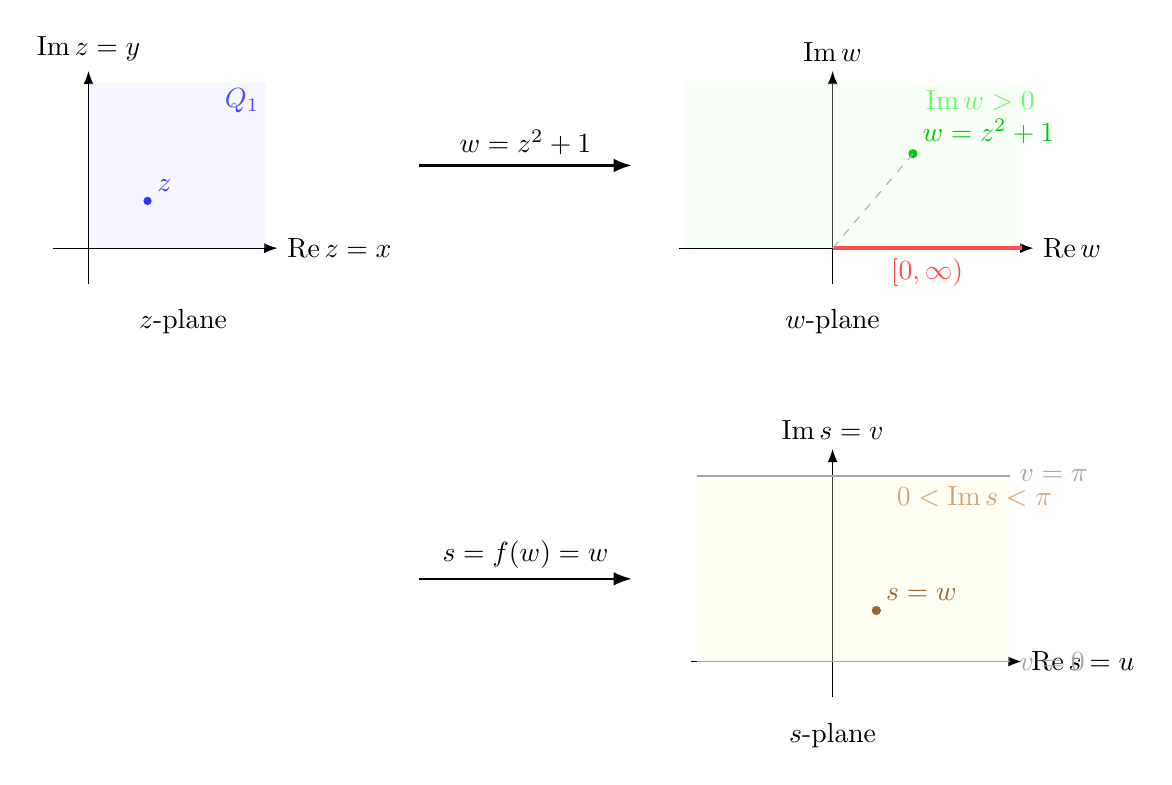
\begin{tikzpicture}[>=Latex,scale=.75]
		% ================= z-plane: domain Q =================
		\begin{scope}
			% axes
			\draw[->] (-0.6,0) -- (3.2,0) node[right] {$\Re z=x$};
			\draw[->] (0,-0.6) -- (0,3.0) node[above] {$\Im z=y$};
			\node at (1.6,-1.25) {$z$-plane};
			
			% shade first quadrant Q: x>0, y>0
			\fill[blue!12, opacity=.25] (0,0) rectangle (3.0,2.8);
			\node[blue!70] at (2.6,2.5) {$Q_1$};
			
			% sample point z = 1 + 0.8 i
			\fill[blue!80] (1.0,0.8) circle (2pt) node[above right] {$z$};
		\end{scope}
		% arrow z -> w
		\draw[->,thick] (5.6,1.4) -- (9.2,1.4) node[midway,above] {$w=z^2+1$};
		% ================= w-plane: image in upper half-plane, slit shown =================
		\begin{scope}[xshift=12.6cm]
			% axes
			\draw[->] (-2.6,0) -- (3.4,0) node[right] {$\Re w$};
			\draw[->] (0,-0.6) -- (0,3.0) node[above] {$\Im w$};
			\node at (0,-1.25) {$w$-plane};
			
			% shade upper half-plane Im w>0
			\fill[green!12, opacity=.25] (-2.5,0) rectangle (3.2,2.8);
			\node[green!60] at (2.5,2.5) {$\Im w>0$};
			
			% slit: [0, +∞) on real axis
			\draw[red!70,very thick] (0,0) -- (3.2,0) node[midway, below] {$[0,\infty)$};
%			\node[gray!70,anchor=west] at (-2.5,-0.35) {$\Omega=\C\setminus[0,\infty)$};
			% image of the sample point: z=1+0.8i -> w=(1-0.64+1)+i(2*1*0.8) = 1.36 + 1.6 i
			\fill[green!80!black] (1.36,1.60) circle (2.2pt) node[above right] {$w=z^2+1$};
			% guide from origin showing |w| and Arg(w)
			\draw[gray!60,dashed] (0,0) -- (1.36,1.60);
%			\node[gray!70] at (0.75,0.18) {$\Arg w\in(0,\pi)$};
		\end{scope}
		% arrow w -> s
		\draw[->,thick] (5.6,1.4-7) -- (9.2,1.4-7) node[midway,above] {$s=f(w)=\Log w$};
		% ================= s-plane: image strip 0<Im s<pi =================
		\begin{scope}[xshift=12.6cm, yshift=-7cm]
			% axes
			\draw[->] (-2.4,0) -- (3.2,0) node[right] {$\Re s=u$};
			\draw[->] (0,-0.6) -- (0,3.6) node[above] {$\Im s=v$};
			\node at (0,-1.25) {$s$-plane};
			% horizontal strip 0 < v < pi
			\fill[yellow!18, opacity=.25] (-2.3,0.00) rectangle (3.0,3.1416);
			\draw[gray!70] (-2.3,0.00) -- (3.0,0.00) node[right] {$v=0$};
			\draw[gray!70] (-2.3,3.1416) -- (3.0,3.1416) node[right] {$v=\pi$};
			\node[brown!70] at (2.4,2.8) {$0<\Im s<\pi$};
			% image of the sample w under Log: s = ln|w| + i Arg(w)
			% |w| ≈ sqrt(1.36^2+1.6^2) ≈ 2.100 -> ln|w| ≈ 0.741, Arg ≈ atan(1.6/1.36) ≈ 0.864
			\fill[brown!80!black] (0.741,0.864) circle (2.2pt)
			node[above right] {$s=\Log w$};
		\end{scope}
%		
%		% ================= footer: analyticity & derivative =================
%		\node[align=left] at (8.6,-0.9)
%		{\small In $Q$: $w=z^2+1$ has $\Im w=2xy>0\Rightarrow w\in\Omega$;\ \ $f=\Log$ is analytic on $\Omega$.\\
%			\small Hence $g(z)=f(z^2+1)$ is analytic on $Q$, and by chain rule
%			$\displaystyle\ g'(z)=f'(z^2+1)\cdot(2z)=\frac{2z}{z^2+1}\,.$};
%		
	\end{tikzpicture}
	\end{center}
	Thus $g$ is the composition of analytic functions on the first quadrant $Q_1$, hence analytic on $Q_1$. By the chain rule, \[
	g'(z)=f'(z^2+1)\cdot(2z)=\frac{2z}{z^2+1}\qquad (z\in Q_1).
	\]
\end{proof}
%	\item Find harmonic conjugates for $u(x,y)=2x-x^3+3xy^2$ and for $u(x,y)=\sinh x\sin y$.
%	\item If $v$ is a harmonic conjugate of $u$ and $u$ a harmonic conjugate of $v$ in $D$, show $u,v$ are constant in $D$.
%	\item Using polar CR, prove that for analytic $f=u+iv$ on $D\subset\C\setminus\{0\}$, $u$ satisfies $r^2u_{rr}+ru_r+u_{\theta\theta}=0$ (polar Laplace equation). Same for $v$.
%	\item Verify $u(r,\theta)=\ln r$ is harmonic on $r>0$, $0<\theta<2\pi$ and $v(r,\theta)=\theta$ is a harmonic conjugate.
%	\item If $f=u+iv$ is analytic on $D$, prove the level curves $u=c_1$ and $v=c_2$ intersect orthogonally at any point where $f'\neq0$.
\end{enumerate}
\newpage





\newpage
\section{Elementary Functions}
\subsection{The Exponential Function}

\defbox[Exponential Function]{
\begin{definition}
	For $z=x+iy\in\C$, define
	\[
	e^z = e^{x+iy} = e^x(\cos y + i\sin y),
	\]
	where $y$ is in radians. We also write $\exp z$ for $e^z$.
\end{definition}}
\thmbox{
\begin{theorem}
	For $z_1,z_2\in\C$,
	\[
	e^{z_1+z_2}=e^{z_1}e^{z_2},\qquad \frac{e^{z_1}}{e^{z_2}}=e^{z_1-z_2}.
	\]
	Moreover, $e^z$ is entire, satisfies \[
	\frac{d}{dz}e^z=e^z
	\] for all $z$, and $e^z\neq 0$ for all $z\in\C$.
\end{theorem}}

\begin{observation}
	Writing $e^z=\rho e^{i\theta}$ gives $\rho=e^x$ and $\theta=y$, hence
	\[
	|e^z|=e^x,\qquad \arg(e^z)=y+2\pi n\ (n\in\mathbb{Z}).
	\]
	Thus $e^{z+2\pi i} = e^z$, so $e^z$ is periodic with pure imaginary period $2\pi i$.
\end{observation}

\corbox[Euler's Identity]{
\begin{corollary}
Euler's identity is given by \[
e^{i\pi}=-1\quad\text{equivalently,}\quad e^{i\pi}+1=0.
\]
\end{corollary}}

\newpage
\begin{example}
Solve $e^z=1+i$ for $z=x+iy$.
\begin{center}
\includegraphics[width=\textwidth]{ca-tikz/chap3-1-2.pdf}
\end{center}
\begin{proof}[\sol]
Since $e^z=e^{x+iy}=e^x(\cos y+i\sin y)$ and $1+i=\sqrt{2}\left(\cos\frac{\pi}{4}+i\sin\frac{\pi}{4}\right)$, we have \[
e^x=\sqrt{2}\quad\text{and}\quad y=\frac{\pi}{4}+2n\pi\quad (n=0,\pm1,\pm2,\cdots).
\] Thus, \[
x=\frac{1}{2}\ln 2\quad\text{and}\quad y=\left(2n+\frac{1}{4}\right)\pi\quad (n=0,\pm1,\pm2,\cdots)
\] and so \[
z=\frac{1}{2}\ln 2 + i\left(2n+\frac{1}{4}\right)\pi\quad (n=0,\pm1,\pm2,\cdots).
\]
\end{proof}	
\end{example}

\newpage
\subsection{The Logarithmic Function}

\begin{observation}
To solve \[
z=e^w
\] for $w$ when $z\neq 0$, write $z=re^{i\theta}$, $w=u+iv$. Then $e^u=r$ and $v=\theta+2\pi n$, hence
\[
\log z = \ln r + i(\theta+2\pi n),\qquad n\in\mathbb{Z},
\]
a multiple-valued function with \[
e^{\log z}=z
\] for $z\neq 0$.
\end{observation}
\begin{center}
	\includegraphics[width=\textwidth]{ca-tikz/chap3-2.pdf}
\end{center}

\begin{example}
If $z=-1-\sqrt3\,i$, then $r=2$ and $\theta=-\tfrac{2\pi}{3}$, so \[
\log z = \ln 2 + i\Bigl(-\tfrac{2\pi}{3} + 2\pi n\Bigr),\quad n\in\mathbb{Z}.
\]
\end{example}

\newpage
\defbox[Argument and Principal Value]{\begin{definition}
For $z\neq 0$, the set of all arguments is $\arg z=\{\theta+2\pi n:n\in\mathbb{Z}\}$ when $z=re^{i\theta}$. The principal value $\Arg z$ is the unique $\theta$ with $-\pi<\theta\le \pi$.
\end{definition}}

\begin{observation}
	In general,
	\[
	\log(e^z)=z+2\pi i\,n,\qquad n\in\mathbb{Z}.
	\]
\end{observation}

\begin{definition}[Principal Value of the Logarithm]
	The principal value is
	\[
	\Log z = \ln r + i\theta\quad (z=re^{i\theta},\ r>0,\ -\pi<\theta<\pi).
	\]
	Then $\log z=\Log z + 2\pi i\,n$ for $n\in\mathbb{Z}$.
\end{definition}

\begin{example}
	$\log 1 = 2\pi i\,n$ with $\Log 1=0$; and $\log(-1)=(2n+1)\pi i$ with $\Log(-1)=\pi i$. The function $\Log z$ is not continuous along the negative real axis.
\end{example}
%
\subsection{Branches and Derivatives of Logarithms}

\begin{observation}
	Let $\alpha\in\R$. Restrict $\theta$ in
	\[
	\log z = \ln r + i\theta\qquad (r>0,\ \alpha<\theta<\alpha+2\pi)
	\]
	to obtain a single-valued continuous branch on that domain; it is in fact analytic there.
\end{observation}

\begin{theorem}
	For a branch as above,
	\[
	\frac{d}{dz}\log z = \frac{1}{z}\qquad(|z|>0,\ \alpha<\arg z<\alpha+2\pi).
	\]
	In particular, on the principal branch,
	\[
	\frac{d}{dz}\Log z = \frac{1}{z}\qquad(|z|>0,\ -\pi<\Arg z<\pi).
	\]
\end{theorem}

\begin{definition}[Branch, Principal Branch, Branch Cut/Point]
	A \emph{branch} of a multiple-valued $f$ is any single-valued analytic function $F$ whose values are among those of $f$. The \emph{principal branch} of $\log$ is $\Log z$ on $r>0$, $-\pi<\theta<\pi$. A \emph{branch cut} is a curve removed to render a single-valued branch; points on it are singular for that branch. The origin is a branch point for $\log$.
\end{definition}

\begin{example}
	$\Log(i^{3})=\Log(-i)=\ln 1 - i\frac{\pi}{2}=-\frac{\pi i}{2}$, while $3\Log i=3\cdot i\frac{\pi}{2}=\frac{3\pi i}{2}$. Hence $\Log(i^{3})\ne 3\Log i$.
\end{example}

\begin{theorem}
	For nonzero $z_1,z_2$,
	\[
	\log(z_1z_2)=\log z_1+\log z_2,\qquad \arg(z_1z_2)=\arg z_1+\arg z_2,
	\]
	and thus $\ln|z_1z_2|+i\arg(z_1z_2)=(\ln|z_1|+i\arg z_1)+(\ln|z_2|+i\arg z_2)$.
\end{theorem}

\begin{example}
	Let $z_1=z_2=-1$. Then $\log 1=0$, while $\log(-1)=(2n+1)\pi i$. Equality can require compatible choices of values. Using principal values everywhere may fail: $\Log(z_1z_2)=0$ but $\Log z_1+\Log z_2=2\pi i$.
\end{example}

\begin{theorem}
	For nonzero $z_1,z_2$,
	\[
	\log\!\left(\frac{z_1}{z_2}\right)=\log z_1-\log z_2.
	\]
\end{theorem}

\begin{observation}[Roots via Logarithm]
	For $z\ne 0$ and $n\in\mathbb{N}$,
	\[
	z^{1/n}=\exp\!\Bigl(\tfrac1n\log z\Bigr),
	\]
	which gives exactly the $n$ distinct $n$th roots when $k=0,1,\dots,n-1$ are taken in the angles.
\end{observation}

\subsection{Complex Exponents}

\begin{definition}[Complex Power]
	For $z\ne 0$ and $c\in\C$,
	\[
	z^{\,c}=e^{c\,\log z},
	\]
	a multiple-valued function in general.
\end{definition}

\begin{example}
	\[
	i^{-2i}=e^{-2i\log i},\qquad \log i = \ln 1 + i\Bigl(\frac{\pi}{2}+2\pi n\Bigr)=\Bigl(2n+\tfrac12\Bigr)\pi i.
	\]
	Hence $i^{-2i}=\exp\!\bigl((4n+1)\pi\bigr)$, which are real numbers.
\end{example}

\begin{observation}
	Since $1/e^z=e^{-z}$, we have $z^{-c}=\exp(-c\log z)$ and in particular $1/i^{2i}=i^{-2i}=\exp\!\bigl((4n+1)\pi\bigr)$.
\end{observation}

\begin{observation}
	Fix a branch $\log z=\ln r+i\theta$ on $\alpha<\theta<\alpha+2\pi$. Then $z^{\,c}=\exp\bigl(c\log z\bigr)$ is single-valued and analytic there, and
	\[
	\frac{d}{dz}z^{\,c}=c\,z^{\,c-1}\qquad(|z|>0,\ \alpha<\arg z<\alpha+2\pi).
	\]
	The principal value is $\mathrm{P.V.}\,z^{\,c}=\exp\bigl(c\,\Log z\bigr)$.
\end{observation}

\begin{example}
	\[
	\mathrm{P.V.}\,(-i)^i=\exp\!\bigl(i\,\Log(-i)\bigr)=\exp\!\left(i\left[\ln 1 - i\frac{\pi}{2}\right]\right)=e^{\pi/2}.
	\]
	For $z^{2/3}$ on the principal branch ($-\pi<\Arg z<\pi$),
	\[
	\mathrm{P.V.}\,z^{2/3}=r^{2/3}\!\left(\cos\frac{2\varphi}{3}+i\sin\frac{2\varphi}{3}\right)\quad(z=re^{i\varphi}).
	\]
\end{example}

\begin{example}
	Let $z_1=1+i$, $z_2=1-i$, $z_3=-1-i$. Then
	\[
	(z_1z_2)^i=e^{i\ln 2},\qquad z_1^{\,i}=e^{-\pi/4}\,e^{i(\ln 2)/2},\qquad z_2^{\,i}=e^{\pi/4}\,e^{i(\ln 2)/2},
	\]
	so $(z_1z_2)^i=z_1^{\,i}z_2^{\,i}$. But
	\[
	(z_2z_3)^i=e^{-\pi}\,e^{i\ln 2},\qquad z_3^{\,i}=e^{3\pi/4}\,e^{i(\ln 2)/2},
	\]
	whence $(z_2z_3)^i = z_2^{\,i}z_3^{\,i}e^{-2i}$, showing branch subtleties.
\end{example}

\begin{definition}[Exponential with Base $c\neq 0$]
	For fixed $c\in\C\setminus\{0\}$ and a chosen value of $\log c$, define
	\[
	c^{\,z}=e^{z\log c}.
	\]
	Then $c^{\,z}$ is entire and $\dfrac{d}{dz}c^{\,z}=c^{\,z}\log c$.
\end{definition}

\subsection{Trigonometric Functions}

\begin{definition}
	For $z\in\C$,
	\[
	\cos z = \frac{e^{iz}+e^{-iz}}{2},\qquad
	\sin z = \frac{e^{iz}-e^{-iz}}{2i}.
	\]
\end{definition}

\begin{theorem}
	The functions $\sin z$ and $\cos z$ are entire and satisfy
	\[
	\frac{d}{dz}\sin z=\cos z,\qquad \frac{d}{dz}\cos z=-\sin z,
	\]
	and remain odd/even respectively: $\sin(-z)=-\sin z$, $\cos(-z)=\cos z$. Moreover $e^{iz}=\cos z + i\sin z$.
\end{theorem}

\begin{theorem}[Formulas]
	For $z,z_1,z_2\in\C$,
	\begin{gather*}
		\sin(z_1+z_2)=\sin z_1\cos z_2+\cos z_1\sin z_2,\quad
		\cos(z_1+z_2)=\cos z_1\cos z_2-\sin z_1\sin z_2,\\
		\sin 2z=2\sin z\cos z,\quad \cos 2z=\cos^2 z-\sin^2 z,\\
		\sin(z+\tfrac{\pi}{2})=\cos z,\quad \cos(z-\tfrac{\pi}{2})=-\cos z,\\
		\sin^2 z+\cos^2 z=1,\quad \sin(z+\pi)=-\sin z,\ \cos(z+\pi)=-\cos z,\\
		\sin(z+2\pi)=\sin z,\quad \cos(z+2\pi)=\cos z.
	\end{gather*}
\end{theorem}

\begin{observation}
	For real $y$,
	\[
	\cos(iy)=\cosh y,\qquad \sin(iy)=i\sinh y.
	\]
	Writing $z=x+iy$,
	\[
	\sin z=\sin x\,\cosh y+i\cos x\,\sinh y,\quad
	\cos z=\cos x\,\cosh y - i\sin x\,\sinh y.
	\]
\end{observation}

\begin{remark}
	$\sin z$ and $\cos z$ are unbounded on $\C$.
\end{remark}

\begin{observation}[Zeros]
	$\sin z=0$ iff $z=n\pi$; $\cos z=0$ iff $z=\frac{\pi}{2}+n\pi$ for $n\in\mathbb{Z}$.
\end{observation}

\begin{definition}
	Define
	\[
	\tan z=\frac{\sin z}{\cos z},\quad \cot z=\frac{\cos z}{\sin z},\quad
	\sec z=\frac{1}{\cos z},\quad \csc z=\frac{1}{\sin z}.
	\]
\end{definition}

\begin{theorem}
	\[
	\frac{d}{dz}\tan z=\sec^2 z,\quad
	\frac{d}{dz}\sec z=\sec z\,\tan z,\quad
	\frac{d}{dz}\cot z=-\csc^2 z,\quad
	\frac{d}{dz}\csc z=-\csc z\,\cot z.
	\]
\end{theorem}

\begin{observation}
	$\tan z$ and $\sec z$ are analytic off $z=\frac{\pi}{2}+n\pi$; $\cot z$ and $\csc z$ are analytic off $z=n\pi$.
\end{observation}

\subsection{Hyperbolic Functions}

\begin{definition}
	\[
	\sinh z=\frac{e^z-e^{-z}}{2},\qquad \cosh z=\frac{e^z+e^{-z}}{2}.
	\]
\end{definition}

\begin{theorem}
	$\sinh z$ and $\cosh z$ are entire and $\dfrac{d}{dz}\sinh z=\cosh z$, $\dfrac{d}{dz}\cosh z=\sinh z$.
\end{theorem}

\begin{theorem}
	For $z=x+iy$ and $z_1,z_2\in\C$,
	\begin{gather*}
		-i\,\sinh(iz)=\sin z,\quad \cosh(iz)=\cos z,\quad
		-i\,\sin(iz)=\sinh z,\quad \cos(iz)=\cosh z,\\
		\sinh(-z)=-\sinh z,\quad \cosh(-z)=\cosh z,\quad
		\cosh^2 z-\sinh^2 z=1,\\
		\sinh(z_1+z_2)=\sinh z_1\cosh z_2+\cosh z_1\sinh z_2,\\
		\cosh(z_1+z_2)=\cosh z_1\cosh z_2+\sinh z_1\sinh z_2,\\
		\sinh z=\sinh x\cos y+i\cosh x\sin y,\\
		\cosh z=\cosh x\cos y+i\sinh x\sin y,\\
		|\sinh z|^2=\sinh^2 x+\sin^2 y,\quad |\cosh z|^2=\cosh^2 x+\cos^2 y.
	\end{gather*}
\end{theorem}

\begin{remark}
	$\sinh z$ and $\cosh z$ are periodic with period $2\pi i$.
\end{remark}

\begin{observation}[Zeros]
	$\sinh z=0$ iff $z=n\pi i$; $\cosh z=0$ iff $z=(\tfrac{\pi}{2}+n\pi)i$ ($n\in\mathbb{Z}$).
\end{observation}

\begin{definition}
	Define $\tanh z=\dfrac{\sinh z}{\cosh z}$ (analytic where $\cosh z\neq 0$). Set $\coth z=1/\tanh z$, $\operatorname{sech}z=1/\cosh z$, $\operatorname{csch}z=1/\sinh z$.
\end{definition}

\begin{theorem}
	\[
	\frac{d}{dz}\tanh z=\operatorname{sech}^2 z,\quad
	\frac{d}{dz}\operatorname{sech}z=-\operatorname{sech}z\,\tanh z,\quad
	\frac{d}{dz}\coth z=-\operatorname{csch}^2 z,\quad
	\frac{d}{dz}\operatorname{csch}z=-\operatorname{csch}z\,\coth z.
	\]
\end{theorem}

\newpage
\subsection{Inverse Trigonometric and Hyperbolic Functions}

\begin{observation}
	To define $\sin^{-1}z$, write \[
	z=\sin w=\dfrac{e^{iw}-e^{-iw}}{2i}.
	\] Then \begin{align*}
		e^{iw}-e^{-iw}&=2iz\\
		(e^{iw})^2-2iz-1&=0\\
	\end{align*} Solving the quadratic in $e^{iw}$ yields
	\[
	e^{iw}=iz+(1-z^2)^{1/2},
	\]
	where $(1-z^2)^{1/2}$ is double-valued.
\end{observation}

\defbox{
\begin{definition}
	Multiple-valued inverses: \begin{align*}
	\sin^{-1}z&=-i\,\log\bigl[\,iz+(1-z^2)^{1/2}\bigr], \\ \\
	\cos^{-1}z&=-i\,\log\bigl[\,z+i(1-z^2)^{1/2}\bigr],\\ \\
	\tan^{-1}z&=\frac{i}{2}\log\!\left(\frac{i+z}{i-z}\right).
	\end{align*}
	With specific branches of $\sqrt{\cdot}$ and $\log$, these become single-valued and analytic on suitable domains.
\end{definition}}
\vfill
\thmbox{
\begin{theorem}[Derivatives]
	\[
	\frac{d}{dz}\sin^{-1}z=\frac{1}{(1-z^2)^{1/2}},\qquad
	\frac{d}{dz}\cos^{-1}z=-\frac{1}{(1-z^2)^{1/2}},\qquad
	\frac{d}{dz}\tan^{-1}z=\frac{1}{1+z^2}.
	\]
\end{theorem}}

\newpage
\begin{example}
	\[
	\sin^{-1}(-i)=-i\,\log\bigl(1\pm\sqrt2\,\bigr).
	\]
	Since $\log(1+\sqrt2)=\ln(1+\sqrt2)+2\pi i\,n$ and $\log(1-\sqrt2)=\ln(\sqrt2-1)+(2n+1)\pi i$ with $\ln(\sqrt2-1)=-\ln(1+\sqrt2)$, the values of $\sin^{-1}(-i)$ are
	\[
	n\pi + i(-1)^{n+1}\ln(1+\sqrt2),\qquad n\in\mathbb{Z}.
	\]
\end{example}

\begin{observation}[Inverse Hyperbolic Functions]
	\[
	\sinh^{-1}z=\log\bigl[z+(z^2+1)^{1/2}\bigr],\quad
	\cosh^{-1}z=\log\bigl[z+(z^2-1)^{1/2}\bigr],\quad
	\tanh^{-1}z=\frac12\log\!\left(\frac{1+z}{1-z}\right).
	\]
\end{observation}

\newpage
\subsection{Exercises}
\begin{exercise}
	Show that $f(z)=\exp(\overline{z})$ is not analytic anywhere. \emph{(Hint: use the Cauchy--Riemann equations.)}
\end{exercise}

\begin{exercise}
	Let $f(z)=u(x,y)+iv(x,y)$ be analytic in a domain $D$. Show that
	\[
	U(x,y)=e^{u(x,y)}\cos v(x,y),\qquad V(x,y)=e^{u(x,y)}\sin v(x,y)
	\]
	are harmonic in $D$, and that $V$ is a harmonic conjugate of $U$.
\end{exercise}

\begin{exercise}
	Show that $f(z)=\Log(z-i)$ is analytic except on the half-line $y=1$, $x\le 0$, and that
	\[
	g(z)=\frac{\Log(z+4)}{z^2+i}
	\]
	is analytic everywhere except at $z=\pm\frac{1-i}{\sqrt2}$ and on the half-line $x\le -4$ on the real axis.
\end{exercise}

\begin{exercise}
	Show that $\ln(x^2+y^2)$ is harmonic in any domain not containing the origin.
\end{exercise}

\begin{exercise}
	Show that neither $\sin z$ nor $\cos z$ is an analytic function of $\overline{z}$ anywhere. \emph{(Hint: Cauchy--Riemann.)}
\end{exercise}

\begin{exercise}
	Show that $\cosh^2 z-\sinh^2 z=1$ and $\sinh z+\cosh z=e^z$.
\end{exercise}


\newpage
\section{Integrals: Part I}

\subsection{Definite Integrals of Complex-Valued Functions}

\defbox[Derivative]{
\begin{definition}\label{def:derivative}
	If $w(t)=u(t)+iv(t)$ with real-valued $u,v$, the derivative is
	\[
	\dv{t}w(t)=w'(t)=u'(t)+iv'(t),
	\]
	whenever $u'$ and $v'$ exist. If $z_0=x_0+iy_0$ is constant, then
	\[
	\dv{t}\big[z_0w(t)\big]=z_0\,w'(t),\qquad
	\dv{t}\,e^{z_0t}=z_0\,e^{z_0t}.
	\]
\end{definition}}

\begin{observation}[No mean value theorem for derivatives]
	If $w(t)$ is continuous on $[a,b]$ and differentiable on $(a,b)$, there need \emph{not} exist $c\in(a,b)$ with
	\[
	w'(c)=\frac{w(b)-w(a)}{b-a}.
	\]
	For $w(t)=e^{it}$ on $[0,2\pi]$, we have $\abs{w'(t)}=1$ but $[w(2\pi)-w(0)]/(2\pi)=0$. 
\end{observation}

\begin{definition}[Definite integral]\label{def:defint}
	For $w(t)=u(t)+iv(t)$,
	\[
	\int_a^b w(t)\,dt
	=\int_a^b u(t)\,dt \;+\; i\int_a^b v(t)\,dt,
	\]
	with analogous definitions for improper integrals.
\end{definition}

\begin{example}
	\[
	\int_0^1 (1+it)^2\,dt
	=\int_0^1(1-t^2)\,dt+i\int_0^1 2t\,dt
	=\frac{2}{3}+i.
	\]
\end{example}

\begin{theorem}[Additivity]
	For $a\le c\le b$,
	\[
	\int_a^b w(t)\,dt=\int_a^c w(t)\,dt+\int_c^b w(t)\,dt.
	\]
\end{theorem}

\newpage
\thmbox[Fundamental Theorem of Calculus]{
\begin{theorem}\label{thm:FTC}
	If $W'(t)=w(t)$ and $W,w$ are continuous on $[a,b]$, then \[
	\int_a^b w(t)\,dt=W(b)-W(a).
	\]
\end{theorem}}
\begin{example}
	Since $\dv{t}\!\big(e^{it}/i\big)=e^{it}$,
	\[
	\int_0^{\pi/4}e^{it}\,dt=\left[\frac{e^{it}}{i}\right]_{0}^{\pi/4}
	=\frac{1}{\sqrt2}+i\!\left(1-\frac{1}{\sqrt2}\right).
	\]
\end{example}

\begin{remark}[No mean value theorem for integrals]
	There need not be $c\in(a,b)$ with \[
	w(c)=\frac{1}{b-a}\int_a^bw(t)\,dt
	\] when $w$ is complex-valued.
\end{remark}

\subsection{Contours}

\defbox[Arc]{
\begin{definition}\label{def:arc}
	An \emph{arc} $C$ is a set $z(t)=x(t)+iy(t)$, $a\le t\le b$, where $x,y$ are continuous.
\end{definition}}

\begin{definition}[Simple arc / Jordan curve]
	$C$ is \emph{simple} if $z(t_1)\ne z(t_2)$ for $t_1\ne t_2$. If $C$ is simple with $z(a)=z(b)$, it is a \emph{simple closed curve} (Jordan curve). Positive orientation is counterclockwise.
\end{definition}

\begin{example}
	The polygonal line from $0$ to $1+i$ to $2+i$ is a simple arc; $z=e^{i\theta}$, $0\le\theta\le2\pi$, is a positively oriented unit circle; $z=z_0+Re^{i\theta}$ is a circle centered at $z_0$ of radius $R$. Traversing $z=e^{-i\theta}$ reverses orientation; $z=e^{i2\theta}$ traverses the unit circle twice.
\end{example}

\begin{observation}[Arc length]
	If $z'(t)=x'(t)+iy'(t)$ is continuous on $[a,b]$, then
	\[
	L(C)=\int_a^b \abs{z'(t)}\,dt,\qquad
	\abs{z'(t)}=\left([x'(t)]^2+[y'(t)]^2\right)^{1/2}.
	\]
	The unit tangent is $T=z'(t)/\abs{z'(t)}$ where $z'(t)\neq0$; such an arc is \emph{smooth}.
\end{observation}

\defbox[Smooth arc and contour]{
\begin{definition}\label{def:contour}
	An arc is \emph{smooth} if $z'(t)$ is continuous on $[a,b]$ and nonzero on $(a,b)$. A \emph{contour} (piecewise smooth arc) is a finite concatenation of smooth arcs. A contour with identical initial and final points is a \emph{simple closed contour}.
\end{definition}}

\thmbox[Jordan Curve Theorem]{
\begin{theorem}
	A simple closed curve $C$ is the boundary of exactly two domains: a bounded interior and an unbounded exterior.
\end{theorem}}

\subsection{Contour Integrals}

\defbox[Contour integral]{
\begin{definition}\label{def:contint}
	If $C$ is given by $z=z(t)$, $a\le t\le b$, and $f$ is (piecewise) continuous on $C$, define
	\[
	\int_C f(z)\,dz \;=\;\int_a^b f(z(t))\,z'(t)\,dt.
	\]
	This is invariant under reparametrization of $C$.
\end{definition}}

\probox[Linearity]{
\begin{proposition}
	For a contour $C$ and constant $z_0$,
	\[
	\int_C z_0 f(z)\,dz=z_0\!\int_C f(z)\,dz,\qquad
	\int_C [f(z)+g(z)]\,dz=\int_C f+\int_C g.
	\]
\end{proposition}}

\probox[Orientation reversal]{
\begin{proposition}
	If $-C$ is $C$ with reversed direction, then
	\[
	\int_{-C} f(z)\,dz = -\int_C f(z)\,dz.
	\]
\end{proposition}}

\probox[Additivity over legs]{
\begin{proposition}
	If $C=C_1+C_2$ (concatenation), then
	\[
	\int_C f(z)\,dz=\int_{C_1} f+\int_{C_2} f.
	\]
\end{proposition}}

\begin{example}[Half-circle integral]
	Let $C:\; z=2e^{i\theta}$, $-\pi/2\le\theta\le\pi/2$ (right half of $\abs{z}=2$). Then
	\[
	\int_C z\,dz
	=\int_{-\pi/2}^{\pi/2} 2e^{i\theta}(2ie^{i\theta})\,d\theta
	=4i\int_{-\pi/2}^{\pi/2} e^{2i\theta}\,d\theta
	=4\pi i.
	\]
\end{example}

\begin{example}[Polygonal and diagonal paths]
	Let $f(z)=y-x- i\,3x^2$ with $z=x+iy$. With $C_1:$ $O\to A\to B$ (up then right) and $C_2:$ $O\to B$ along $y=x$, one finds
	\[
	\int_{C_1}\!f(z)\,dz=\frac{1-i}{2},\qquad
	\int_{C_2}\!f(z)\,dz=1-i,\qquad
	\int_{C_1-C_2}\!f(z)\,dz=\frac{-1+i}{2}.
	\]
\end{example}

\begin{example}[Path-independence for $f(z)=z$]
	For any smooth arc $C$ from $z_1$ to $z_2$,
	\[
	\int_C z\,dz=\frac{z_2^2-z_1^2}{2}.
	\]
	Hence the value depends only on endpoints, so the same holds for any piecewise smooth contour by telescoping the legs.
\end{example}

\begin{example}[Square-root branch on a semicircle]
	Let $C:\; z=3e^{i\theta}$, $0\le\theta\le\pi$ and take the branch $z^{1/2}=\exp\big(\tfrac12\log z\big)$ on $\abs{z}>0$, $0<\arg z<2\pi$. Then $z^{1/2}$ is piecewise continuous on $C$ and
	\[
	\int_C z^{1/2}\,dz
	=3\sqrt{3}\,i\int_0^{\pi} e^{i(3\theta/2)}\,d\theta
	=-2\sqrt3\,(1+i).
	\]
\end{example}

\begin{example}[Power integral on a circle]
	On the principal branch $z^{a-1}=\exp[(a-1)\Log z]$ with $\abs{z}>0$, $-\pi<\Arg z<\pi$, for $C:\; z=Re^{i\theta}$, $-\pi<\theta<\pi$,
	\[
	\int_C z^{a-1}\,dz
	=iR^{a}\!\int_{-\pi}^{\pi} e^{ia\theta}\,d\theta
	=\frac{i\,2R^{a}}{a}\,\sin(a\pi).
	\]
	If $a=n\in\mathbb{Z}\setminus\{0\}$, this vanishes; for $a=0$ it yields
	\[
	\int_C \frac{1}{z}\,dz
	=\int_{-\pi}^{\pi} \frac{i\,Re^{i\theta}}{Re^{i\theta}}\,d\theta
	=2\pi i.
	\]
\end{example}

\newpage
\subsection{Upper Bounds for Moduli of Contour Integrals}

\lembox{
\begin{lemma}\label{lem:scalarbound}
	If $w(t)$ is piecewise continuous on $[a,b]$, then
	\[
	\left|\int_a^b w(t)\,dt\right|\le \int_a^b \abs{w(t)}\,dt.
	\]
\end{lemma}}

\thmbox[ML-inequality]{
\begin{theorem}\label{thm:ML}
	Let $C$ be a contour of length $L=b-a$, and suppose $f$ is piecewise continuous on $C$ with $\abs{f(z)}\le M$ on $C$. Then
	\[
	\left|\int_C f(z)\,dz\right|\le ML(=M(b-a)).
	\]
\end{theorem}}

\begin{example}
	On the quarter-circle $C:\abs{z}=2$ from $2$ to $2i$,
	\[
	\left|\int_C \frac{z+4}{z^3-1}\,dz\right|
	\le \frac{6}{7}\cdot \frac{\pi}{2}\cdot 2
	= \frac{6\pi}{7},
	\]
	since $\abs{z+4}\le6$, $\abs{z^3-1}\ge7$, and $L=\pi$.
\end{example}

\begin{example}[Large semicircle vanishing]
	Let $C_R:\; z=Re^{i\theta}$, $0\le\theta\le\pi$, and take $z^{1/2}=\exp\big(\tfrac12\log z\big)$ on $\abs{z}>0$, $-\pi/2<\theta<3\pi/2$. Then
	\[
	\left|\int_{C_R}\frac{z^{1/2}}{z^2+1}\,dz\right|
	\le \max_{C_R}\frac{\sqrt{R}}{R^2-1}\cdot (\pi R)
	=\frac{\pi R\sqrt{R}}{R^2-1}\xrightarrow[R\to\infty]{}0.
	\]
	Hence $\displaystyle \lim_{R\to\infty}\int_{C_R}\frac{z^{1/2}}{z^2+1}\,dz=0$.
\end{example}

\subsection{Antiderivatives and Path Independence}

\thmbox{
\begin{theorem}\label{thm:anti-equivalences}
	Let $f$ be continuous on a domain $D\subset\C$. The following are equivalent:
	\begin{enumerate}[(1)]
		\item $f$ has an antiderivative $F$ on $D$;
		\item For any $z_1,z_2\in D$ and any contour $C$ in $D$ from $z_1$ to $z_2$,
		\[
		\int_C f(z)\,dz=F(z_2)-F(z_1);
		\]
		\item $\displaystyle \int_C f(z)\,dz=0$ for every closed contour $C$ in $D$.
	\end{enumerate}
\end{theorem}}

\begin{example}
	$f(z)=z^2$ has antiderivative $F(z)=z^3/3$ on $\C$; thus for any contour $0\to 1+i$,
	\[
	\int_0^{1+i} z^2\,dz=\left[\frac{z^3}{3}\right]_0^{1+i}
	=\frac{2}{3}(-1+i).
	\]
\end{example}

\begin{example}
	$f(z)=z^{-2}$ is continuous on $\C\setminus\{0\}$ with antiderivative $F(z)=-1/z$ on $\abs{z}>0$. Therefore for the circle $z=2e^{i\theta}$,
	\[
	\int_{|z|=2}\frac{1}{z^2}\,dz=0.
	\]
\end{example}

\begin{example}[Using branches of $\log$ for $1/z$]
	On the right semicircle $C_1:\; z=2e^{i\theta}$, $-\pi/2\le\theta\le\pi/2$, the principal branch
	\[
	\Log z=\ln r + i\varphi\quad (r>0,\ -\pi<\varphi<\pi)
	\]
	is an antiderivative of $1/z$, hence
	\[
	\int_{C_1}\frac{1}{z}\,dz=\Log(2i)-\Log(-2i)=\pi i.
	\]
	On the left semicircle $C_2:\; \pi/2\le\theta\le 3\pi/2$ using the branch
	\[
	\log z=\ln r + i\theta\quad (r>0,\ 0<\theta<2\pi),
	\]
	we likewise obtain
	\[
	\int_{C_2}\frac{1}{z}\,dz=\log(-2i)-\log(2i)=\pi i.
	\]
	Therefore $\displaystyle \oint_{|z|=2}\frac{1}{z}\,dz=2\pi i$.
\end{example}

%\vspace{1em}
%\noindent\textbf{References.} Content adapted from the provided lecture slides for \emph{Complex Variables and Applications, Chapter 4: Integrals (Part I)}. :contentReference[oaicite:0]{index=0}
%

\newpage
\section{Integrals: Part II}
\subsection{Cauchy--Goursat Theorem}

We begin with the real-variable result which motivates Cauchy's theorem.
\thmbox[Green's Theorem]{\label{thm:greens}
\begin{theorem}
Let $C(=\partial R)$ be a positively oriented simple closed contour in the plane, and let $R$ be the region it encloses. Suppose $P(x,y),Q(x,y)$ are continuous on $C\cup R$ and have continuous first partial derivatives $P_x,P_y,Q_x,Q_y$ there. Then \[
\int_{C=\partial R} P(x,y)\,\d x + Q(x,y)\,\d y = \iint_R \left(\frac{\partial Q}{\partial x} - \frac{\partial P}{\partial y}\right)\,\d x\,\d y = \iint_R \left(\frac{\partial Q}{\partial x} - \frac{\partial P}{\partial y}\right)\,\d A.
\]
\end{theorem}}
This gives rise to one of the central theorems of complex integration.

\thmbox[Cauchy's Theorem (elementary form)]{
\begin{theorem}
Let $f$ be analytic and $f'$ continuous in a simply connected domain $D\subset\C$. If $C$ is a positively oriented simple closed contour in $D$, then \[
\int_C f(z)\,dz = 0.
\]
\end{theorem}}
\begin{remark}
	Let $f=u+iv$ and $z=z(t)=x(t)+iy(t)$ ($\d z=dx+idy$). Then \begin{align*}
		\int f(z)\d z &= \int (u\d x - v\d y+i(vdx+u \d y))\\
		&= \int (udx-vdy)+i\int(vdx+udy) \\
		&= \iint_D
	\end{align*}
\end{remark}

\begin{example}
	Let $C$ be any simple closed contour. The function $f(z)=e^{z^3}$ is entire. Hence
	\[
	\int_C e^{z^3}\,dz = 0.
	\]
\end{example}

\newpage\noindent
To remove the hypothesis ``$f'$ is continuous'', we use a covering lemma.

%\lembox{[Covering Lemma]{
\begin{lemma}\label{lem:cover}
	Let $f$ be analytic throughout a closed region $R$ consisting of the interior of a positively oriented simple closed contour $C$ together with the points of $C$ itself. For any $\varepsilon>0$, the region $R$ can be covered by finitely many (possibly partial) squares indexed by $j=1,\dots,n$ such that in each square there is a point $z_j$ with
	\[
	\left| \frac{f(z)-f(z_j)}{z-z_j} - f'(z_j) \right| < \varepsilon
	\]
	for all $z$ in that square distinct from $z_j$.
\end{lemma}
%}

\thmbox[Cauchy--Goursat Theorem]{
\begin{theorem}\label{thm:CG}
If $f$ is analytic at all points on and inside a positively oriented simple closed contour $C$, then
\[
\int_C f(z)\,dz = 0.
\]
\end{theorem}}

\subsection{Integrals on Simply and Multiply Connected Domains}

\defbox[Simply connected domain]{
\begin{definition}
	A domain $D\subset\C$ is \emph{simply connected} if every simple closed contour contained in $D$ encloses only points of $D$ (equivalently: any closed contour in $D$ can be continuously deformed to a point while remaining in $D$).
\end{definition}}

\begin{example}
	The interior of a simple closed curve is simply connected. The annulus
	\[
	\{z: r<|z|<R\}
	\]
	is not simply connected because closed contours can wind around the missing center point.
\end{example}

\begin{definition}[Multiply connected domain]
	A domain that is not simply connected is called \emph{multiply connected}.
\end{definition}

\thmbox[Cauchy on simply connected domains]{
\begin{theorem}\label{thm:simple}
	If $f$ is analytic throughout a simply connected domain $D$, then
	\[
	\int_C f(z)\,dz = 0
	\]
	for every closed contour $C$ contained in $D$.
\end{theorem}}

\begin{example}
	Let $C$ be any closed contour in the disk $\{z:|z|<2\}$. Consider
	\[
	f(z) = \frac{z e^z}{(z^2+9)^5}.
	\]
	The poles at $z=\pm 3i$ lie outside $|z|<2$. On $|z|<2$ the function $f$ is analytic. Hence
	\[
	\int_C \frac{z e^z}{(z^2+9)^5}\,dz = 0.
	\]
\end{example}

The following result ties together antiderivatives, path-independence, and zero integral over closed contours.

\begin{theorem}[Equivalence]\label{thm:equiv}
	Let $f$ be continuous on a domain $D$. The following are equivalent:
	\begin{enumerate}
		\item $f$ has an antiderivative $F$ on $D$;
		\item For any $z_1,z_2\in D$, and any contour $C$ in $D$ from $z_1$ to $z_2$,
		\[
		\int_C f(z)\,dz = F(z_2)-F(z_1);
		\]
		\item For every closed contour $C$ in $D$,
		\[
		\int_C f(z)\,dz = 0.
		\]
	\end{enumerate}
\end{theorem}

\begin{corollary}
	If $f$ is analytic throughout a simply connected domain $D$, then $f$ has an antiderivative on $D$.
\end{corollary}

\begin{remark}
	Since the entire plane $\C$ is simply connected, every entire function possesses an entire antiderivative.
\end{remark}

\subsubsection*{Multiply connected case}
\thmbox[Cauchy for multiply connected regions]{
\begin{theorem}\label{thm:mult}
	Suppose
	\begin{enumerate}
		\item $C$ is a positively oriented simple closed contour;
		\item $C_1,\dots,C_n$ are negatively oriented (clockwise) simple closed contours interior to $C$, pairwise disjoint, and their interiors do not intersect;
		\item $f$ is analytic on $C$, on each $C_k$, and on the region consisting of points inside $C$ and outside all $C_k$.
	\end{enumerate}
	Then
	\[
	\int_C f(z)\,dz + \sum_{k=1}^n \int_{C_k} f(z)\,dz = 0.
	\]
\end{theorem}}

\corbox[Deformation of Paths]{
\begin{corollary}
	Let $C_1$ and $C_2$ be positively oriented simple closed contours with $C_1$ inside $C_2$. If $f$ is analytic on and between these contours, then
	\[
	\int_{C_1} f(z)\,dz = \int_{C_2} f(z)\,dz.
	\]
\end{corollary}}

\begin{example}
	Let $C$ be any positively oriented simple closed contour around the origin. Then
	\[
	\int_C \frac{1}{z}\,dz = 2\pi i.
	\]
	Indeed, by deformation we may replace $C$ by the unit circle.
\end{example}

\newpage
\subsection{Cauchy Integral Formula}

We now reach one of the most powerful formulas in complex analysis.
\thmbox[Cauchy Integral Formula]{
\begin{theorem}\label{thm:CIF}
Let $f$ be analytic on and inside a positively oriented simple closed contour $C$, and let $z_0$ be a point interior to $C$. Then \[
f(z_0) = \frac{1}{2\pi i} \int_C \frac{f(z)}{z - z_0}\,dz.
\]
\end{theorem}}
\begin{remark}
\begin{align*}
\int_C \frac{f(z)}{z - z_0}\,dz&=\int_C\frac{f(z)-f(z_0)+f(z_0)}{z-z_0}\\
&=\int_C \frac{f(z)-f(z_0)}{z - z_0}\,dz+\int_C \frac{f(z_0)}{z - z_0}\,dz
\end{align*}
\end{remark}

\begin{remark}
	This formula shows that the values of $f$ inside $C$ are \emph{completely determined} by the values of $f$ on $C$.
\end{remark}

\begin{observation}
	Written as
	\[
	\int_C \frac{f(z)}{z - z_0}\,dz = 2\pi i\,f(z_0),
	\]
	the formula is very convenient for evaluating contour integrals.
\end{observation}

\begin{example}
	Let $C$ be the positively oriented circle $|z|=2$. Consider
	\[
	\int_C \frac{z}{(9 - z^2)(z + i)}\,dz.
	\]
	Write $f(z)=\dfrac{z}{9 - z^2}$, which is analytic on $|z|\le 2$, and $z_0 = -i$ lies inside $C$. Then
	\[
	\int_C \frac{f(z)}{z - (-i)}\,dz
	= 2\pi i\, f(-i)
	= 2\pi i \cdot \frac{-i}{9 - (-i)^2}
	= 2\pi i \cdot \frac{-i}{9+1}
	= \frac{\pi}{5}.
	\]
\end{example}

\subsubsection{Cauchy formulas for derivatives}
\thmbox[Cauchy formula for $f'$]{
\begin{theorem}
	Under the hypotheses of Theorem~\ref{thm:CIF}, for $z$ interior to $C$,
	\[
	f'(z) = \frac{1}{2\pi i} \int_C \frac{f(s)}{(s - z)^2}\,ds.
	\]
\end{theorem}}
\begin{remark}
\begin{align*}
	f(z)-\frac{1}{2\pi i}\int_C\frac{f(s)}{s-z}dz &\implies f'(z)=\frac{df}{dz}=\frac{d}{dz}\left(\frac{1}{2\pi i}\int_C\frac{f(s)}{s-z}\ ds\right)
\end{align*}
\end{remark}

\corbox[Cauchy formula for higher derivatives]{
\begin{corollary}
If $f$ is analytic on and inside $C$, then for $n=1,2,\dots$,
\[
f^{(n)}(z) = \frac{n!}{2\pi i} \int_C \frac{f(s)}{(s - z)^{n+1}}\,ds.
\]
Equivalently,
\[
\int_C \frac{f(s)}{(s - z)^{n+1}}\,ds = \frac{2\pi i}{n!} f^{(n)}(z).
\]
\end{corollary}}

\begin{example}
	Let $C$ be the positively oriented unit circle $|z|=1$. Evaluate
	\[
	\int_C \frac{e^{2z}}{z^4}\,dz.
	\]
	Here $f(z)=e^{2z}$ is analytic everywhere and we want the coefficient corresponding to $(s-0)^{-4}$. Take $z=0$ and $n=3$ in the corollary:
	\[
	\int_C \frac{f(s)}{s^{4}}\,ds
	= \frac{2\pi i}{3!} f^{(3)}(0).
	\]
	But $f^{(3)}(z) = 2^3 e^{2z} = 8 e^{2z}$, so $f^{(3)}(0)=8$. Hence
	\[
	\int_C \frac{e^{2z}}{z^4}\,dz = \frac{2\pi i}{6}\cdot 8 = \frac{8\pi i}{3}.
	\]
\end{example}

\begin{example}
	Let $f(z)=1$. Then
	\[
	\int_C \frac{1}{z-z_0}\,dz = 2\pi i,\qquad
	\int_C \frac{1}{(z-z_0)^{n+1}}\,dz = 0,\quad n=1,2,\dots
	\]
	whenever $z_0$ is inside $C$.
\end{example}

\newpage
\subsection{Consequences of the Cauchy Integral Formula}
\subsubsection{Analyticity of derivatives}
\thmbox{\begin{theorem}
	If $f$ is analytic at a point $z_0$, then all derivatives $f^{(n)}$ exist and are analytic at $z_0$.
\end{theorem}}

\corbox{
\begin{corollary}
	If $f(z)=u(x,y)+iv(x,y)$ is analytic at $z_0$, then $u$ and $v$ have continuous partial derivatives of all orders in a neighborhood of $z_0$.
\end{corollary}}

\subsection{Morera's Theorem}

\begin{theorem}[Morera]\label{thm:morera}
	Let $f$ be continuous on a domain $D$. If
	\[
	\int_C f(z)\,dz = 0
	\]
	for every closed contour $C$ in $D$, then $f$ is analytic throughout $D$.
\end{theorem}

\subsubsection{Cauchy's Inequalities}

\begin{theorem}[Cauchy's inequality]\label{thm:cauchyineq}
	Suppose $f$ is analytic on and inside the circle $C_R=\{z:|z-z_0|=R\}$, and let
	\[
	M_R = \max_{|z-z_0|=R} |f(z)|.
	\]
	Then for $n=0,1,2,\dots$,
	\[
	|f^{(n)}(z_0)| \le \frac{n!\, M_R}{R^n}.
	\]
\end{theorem}

\newpage
\subsection{Liouville's Theorem and the Fundamental Theorem of Algebra}
\thmbox[Liouville]{
\begin{theorem}\label{thm:liouville}
	If $f$ is entire and bounded in the whole complex plane, then $f$ is constant.
\end{theorem}}

\thmbox[Fundamental Theorem of Algebra]{
\begin{theorem}\label{thm:FTA}
	Let
	\[
	P(z)=a_0+a_1 z + \dots + a_n z^n,\qquad a_n\neq 0,\ n\ge 1,
	\]
	be a complex polynomial. Then $P$ has at least one zero in $\C$.
\end{theorem}}

\begin{remark}
	It follows that any polynomial of degree $n$ can be factored into linear factors:
	\[
	P(z)=c(z-z_1)(z-z_2)\cdots(z-z_n),\qquad c,z_k\in\C.
	\]
\end{remark}

\subsection{Maximum Modulus Principle}

\begin{lemma}
	Suppose $f$ is analytic in a disk $|z-z_0|<\varepsilon$ and $|f(z)|\le |f(z_0)|$ for all such $z$. Then $f$ is constant in that disk.
\end{lemma}

\begin{theorem}[Maximum Modulus Principle]\label{thm:MMP}
	If $f$ is analytic and non-constant in a domain $D$, then $|f(z)|$ has no maximum value in $D$.
\end{theorem}

\begin{corollary}
	Let $f$ be continuous on a closed bounded region $R$, analytic and non-constant on the interior of $R$. Then $\max_{z\in R} |f(z)|$ is attained on the boundary of $R$, not in the interior.
\end{corollary}

\begin{remark}
	If $f=u+iv$ is analytic, then $u$ is harmonic. The corollary implies a maximum principle for $u$ as well.
\end{remark}

\begin{example}
	Let $R=\{0\le x\le \pi,\ 0\le y\le 1\}$ and $f(z)=\sin z$. Since
	\[
	\sin z = \sin x \cosh y + i \cos x \sinh y,
	\]
	we have
	\[
	|f(z)|^2 = \sin^2 x + \sinh^2 y.
	\]
	On $R$, $\sin^2 x$ is largest at $x=\pi/2$ and $\sinh^2 y$ is largest at $y=1$, so the maximum of $|f(z)|$ on $R$ is attained at $z=\pi/2 + i$ and nowhere in the interior.
\end{example}

%\section{Exercises}
%
%\begin{enumerate}[label=\textbf{E\arabic*.}]
%	\item Let $C_0$ be the positively oriented circle $|z-z_0|=R$. Show that
%	\[
%	\int_{C_0} (z - z_0)^{n-1}\,dz =
%	\begin{cases}
%		0, & n=\pm1,\pm2,\dots, \ n\ne 0,\\[2pt]
%		2\pi i, & n=0.
%	\end{cases}
%	\]
%	\item Let $C$ be the boundary of the square with sides $x=\pm 2$, $y=\pm 2$, oriented positively. Show that
%	\[
%	\int_C \frac{\cos z}{z(z^2+8)}\,dz = \frac{i\pi}{4},\qquad
%	\int_C \frac{\cosh z}{z^4}\,dz = 0,
%	\]
%	and, for $-2<x_0<2$,
%	\[
%	\int_C \frac{\tan(z/2)}{(z-x_0)^2}\,dz = i\pi \sec^2\!\left(\frac{x_0}{2}\right).
%	\]
%	\item Let $C$ be the circle $|z|=3$, positively oriented, and define
%	\[
%	f(z)=\int_C \frac{2s^2 - s - 2}{s - z}\,ds,\qquad |z|\ne 3.
%	\]
%	Show that $f(2)=8\pi i$.
%	\item Let $C$ be any positively oriented simple closed contour and
%	\[
%	f(z)=\int_C \frac{s^3 + 2s}{(s - z)^3}\,ds.
%	\]
%	Show that $f(z)=6\pi i\, z$ when $z$ is inside $C$, and $f(z)=0$ when $z$ is outside.
%	\item Let $C$ be the unit circle $z=e^{i\theta}$, $-\pi\le\theta\le\pi$. Show that for any constant $a$,
%	\[
%	\int_C \frac{e^{az}}{z}\,dz = 2\pi i,
%	\]
%	and hence
%	\[
%	\int_0^\pi e^{a\cos\theta} \cos(a\sin\theta)\,d\theta = \pi.
%	\]
%\end{enumerate}
%
%\vspace{1em}
%\noindent Source: lecture note \emph{Complex Variables and Applications, Chapter 4: Integrals (Part II)}. :contentReference[oaicite:0]{index=0}

\section{Series}

\subsection{Convergence of Sequences}

\begin{definition}[Limit of a sequence]
	A sequence $(z_n)$ of complex numbers converges to $z\in\C$ if for each $\varepsilon>0$ there exists $N\in\mathbb{N}$ such that
	\[
	|z_n-z|<\varepsilon\qquad(n>N).
	\]
	We write $\lim_{n\to\infty} z_n=z$. If no such $z$ exists, the sequence \emph{diverges}.
\end{definition}

\begin{remark}[Uniqueness]
	A complex sequence has at most one limit.
\end{remark}

\begin{theorem}[Componentwise convergence]
	Let $z_n=x_n+i y_n$ and $z=x+iy$. Then
	\[
	\lim_{n\to\infty} z_n=z
	\quad\Longleftrightarrow\quad
	\lim_{n\to\infty} x_n=x\ \ \text{and}\ \ \lim_{n\to\infty} y_n=y.
	\]
\end{theorem}

\begin{example}
	(a) $z_n=\dfrac{1}{n^3}+i \ \Rightarrow\ \lim z_n=i$. \quad
	(b) $z_n=-2+i\dfrac{(-1)^n}{n^2}\ \Rightarrow\ \lim z_n=-2$.
\end{example}

\begin{observation}[Polar view]
	Writing $z_n=r_n e^{i\theta_n}$ with $r_n=|z_n|$ and $\theta_n=\Arg z_n$, one may have $r_n\to r$ while $(\theta_n)$ fails to converge (e.g.\ even/odd subsequences approaching $\pm\pi$).
\end{observation}

\newpage
\subsection{Convergence of Series}
\defbox[Series and sum]{
\begin{definition}
	A series $\sum_{n=1}^{\infty} z_n$ converges to $S$ if the partial sums $S_N=\sum_{n=1}^{N} z_n$ satisfy $S_N\to S$. Then $\sum_{n=1}^\infty z_n=S$.
\end{definition}}

\thmbox[Componentwise]{
\begin{theorem}
If $z_n=x_n+i y_n$ and $S=X+iY$, then \[
\sum_{n=1}^{\infty} z_n=S
\quad\Longleftrightarrow\quad
\sum_{n=1}^{\infty} x_n=X\ \ \text{and}\ \ \sum_{n=1}^{\infty} y_n=Y.
\]
\end{theorem}}

\begin{remark}[Necessary test and boundedness]
	If $\sum z_n$ converges, then $z_n\to0$ (the $n$th-term test). In particular, the terms are bounded: there exists $M$ with $|z_n|\le M$ for all $n$.
\end{remark}

\begin{definition}[Absolute convergence]
	$\sum z_n$ is \emph{absolutely convergent} if $\sum |z_n|$ converges. Absolute convergence implies convergence.
\end{definition}

\begin{remark}[Remainders]
	If $S=\sum_{n=1}^\infty z_n$, the remainder after $N$ terms is $\rho_N=S-S_N$. Then $S_N\to S$ iff $\rho_N\to 0$.
\end{remark}

\subsection{Power Series and Taylor Series}
\defbox[Power series centered at $z_0$]{
\begin{definition}
	\[
	\sum_{n=0}^{\infty} a_n (z-z_0)^n=a_0+a_1(z-z_0)+a_2(z-z_0)^2+\cdots,
	\]
	with $a_n,z_0\in\C$.
\end{definition}}

\thmbox[Taylor series]{
\begin{theorem}\label{thm:Taylor}
	If $f$ is analytic on $|z-z_0|<R_0$, then for $|z-z_0|<R_0$,
	\[
	f(z)=\sum_{n=0}^{\infty} a_n (z-z_0)^n,\qquad a_n=\frac{f^{(n)}(z_0)}{n!}.
	\]
	For $z_0=0$ this is the \emph{Maclaurin series}.
\end{theorem}}

\begin{example}
	Since $e^z$ is entire,
	\[
	e^z=\sum_{n=0}^{\infty}\frac{z^n}{n!},\qquad
	z^2 e^{3z}=\sum_{n=0}^{\infty}\frac{3^{\,n-2}}{(n-2)!}\,z^{n}\quad(\text{interpreting }(n-2)!=\infty \text{ for }n<2\text{ gives zero terms}).
	\]
	Also
	\[
	\sin z=\sum_{n=0}^{\infty}\frac{(-1)^n z^{2n+1}}{(2n+1)!},\quad
	\cos z=\sum_{n=0}^{\infty}\frac{(-1)^n z^{2n}}{(2n)!},
	\]
	\[
	\sinh z=\sum_{n=0}^{\infty}\frac{z^{2n+1}}{(2n+1)!},\quad
	\cosh z=\sum_{n=0}^{\infty}\frac{z^{2n}}{(2n)!}.
	\]
\end{example}

\begin{example}[Geometric series]
	For $f(z)=\dfrac{1}{1-z}$ we have
	\[
	\frac{1}{1-z}=\sum_{n=0}^{\infty} z^n,\qquad |z|<1,
	\]
	and similarly $\dfrac{1}{1+z}=\sum_{n=0}^{\infty}(-1)^n z^n$ for $|z|<1$.
\end{example}

\subsection{Laurent Series}

\begin{remark}
	At a point $z_0$ where $f$ is not analytic, Taylor series may fail; on an annulus $R_1<|z-z_0|<R_2$ one often has a two-sided power expansion (Laurent series).
\end{remark}

\begin{theorem}[Laurent]\label{thm:Laurent}
	If $f$ is analytic on the annulus $R_1<|z-z_0|<R_2$ and $C$ is any positively oriented simple closed contour around $z_0$ lying in that annulus, then on $R_1<|z-z_0|<R_2$,
	\[
	f(z)=\sum_{n=0}^{\infty} a_n (z-z_0)^n+\sum_{n=1}^{\infty} \frac{b_n}{(z-z_0)^n}
	=\sum_{n=-\infty}^{\infty} c_n (z-z_0)^n,
	\]
	with
	\[
	c_n=\frac{1}{2\pi i}\int_C \frac{f(\zeta)}{(\zeta-z_0)^{n+1}}\,d\zeta\qquad (n\in\mathbb{Z}).
	\]
	If $f$ is analytic on $|z-z_0|<R_2$ then $b_n=0$ and Laurent reduces to Taylor.
\end{theorem}

\begin{example}
	Since $e^z=\sum_{n=0}^\infty \dfrac{z^n}{n!}$ for all $z$, we get
	\[
	e^{1/z}=\sum_{n=0}^{\infty}\frac{1}{n!}\,\frac{1}{z^n},\qquad 0<|z|<\infty.
	\]
	The coefficient of $(z^{-1})$ is $1$, hence for any positively oriented simple closed contour $C$ around $0$,
	\[
	\int_C e^{1/z}\,dz = 2\pi i.
	\]
\end{example}

\begin{example}[Partial fractions across annuli]
	Let
	\[
	f(z)=\frac{-1}{(z-1)(z-2)}=\frac{1}{z-1}-\frac{1}{z-2}.
	\]
	Three Laurent expansions in powers of $z$ arise:
	\begin{align*}
		|z|<1:&\quad f(z)= -\sum_{n=0}^{\infty} z^{n}+\sum_{n=0}^{\infty}\frac{z^{n}}{2^{\,n+1}}
		= \sum_{n=0}^{\infty}\Big(\frac{1}{2^{\,n+1}}-1\Big) z^{n},\\[2pt]
		1<|z|<2:&\quad f(z)= \sum_{n=0}^{\infty}\frac{1}{z^{n+1}}+\sum_{n=0}^{\infty}\frac{z^{n}}{2^{\,n+1}}
		= \sum_{n=1}^{\infty}\frac{1}{z^{n}}+\sum_{n=0}^{\infty}\frac{z^{n}}{2^{\,n+1}},\\[2pt]
		|z|>2:&\quad f(z)= \sum_{n=1}^{\infty}\frac{1-2^{\,n-1}}{z^{n}}.
	\end{align*}
\end{example}

%\begin{example}
%	Find the Laurent series
%\end{example}

\subsection{Absolute and Uniform Convergence of Power Series}

\begin{theorem}[Absolute convergence inside any interior circle]
	If a power series $\sum_{n=0}^{\infty} a_n (z-z_0)^n$ converges at some $z_1\ne z_0$, then it converges absolutely for all $|z-z_0|<|z_1-z_0|$.
\end{theorem}

\begin{definition}[Circle of convergence]
	The largest open disk centered at $z_0$ on which the series converges is the \emph{circle of convergence}. Its radius is the \emph{radius of convergence}.
\end{definition}

\begin{theorem}[Uniform convergence on closed interior disks]
	If $|z_1-z_0|=R_1$ lies strictly inside the circle $|z-z_0|=R$, then the series is uniformly convergent on the closed disk $|z-z_0|\le R_1$.
\end{theorem}

\subsection{Consequences for Sums of Power/Laurent Series}
$\wedge$
\begin{theorem}[Continuity and analyticity]\label{thm:cont-anal}
	Inside the circle of convergence, the sum $S(z)=\sum_{n=0}^{\infty} a_n (z-z_0)^n$ is continuous and analytic.
\end{theorem}

\begin{remark}[Exterior series]
	If $\sum_{n=1}^{\infty} \dfrac{b_n}{(z-z_0)^n}$ converges at $z_1\ne z_0$, then it converges absolutely to a continuous function on $\{|z-z_0|>|z_1-z_0|\}$ (the exterior of the circle through $z_1$).
\end{remark}

\begin{remark}[Laurent on annuli]
	If
	\[
	f(z)=\sum_{n=0}^{\infty} a_n (z-z_0)^n+\sum_{n=1}^{\infty}\frac{b_n}{(z-z_0)^n}
	\]
	is valid on $R_1<|z-z_0|<R_2$, then both series converge uniformly on any closed annulus $R_1+\varepsilon \le |z-z_0|\le R_2-\varepsilon$ ($\varepsilon>0$).
\end{remark}

\begin{theorem}[Termwise integration on interior contours]
	Let $C$ be a contour inside the circle of convergence of $\sum_{n=0}^{\infty} a_n (z-z_0)^n$ and $f$ continuous on $C$. Then
	\[
	\int_C f(z)\,\sum_{n=0}^{\infty} a_n (z-z_0)^n\,dz
	=\sum_{n=0}^{\infty} a_n \int_C f(z)(z-z_0)^n\,dz.
	\]
\end{theorem}

\begin{corollary}
	The sum $S(z)$ is analytic inside its circle of convergence and may be integrated term by term on interior contours.
\end{corollary}

\begin{example}
	Define
	\[
	f(z)=
	\begin{cases}
		\dfrac{e^{z}-1}{z},& z\ne 0,\\[4pt]
		1,& z=0.
	\end{cases}
	\]
	Since $e^{z}-1=\sum_{n=1}^\infty \dfrac{z^{n}}{n!}$, we obtain $f(z)=\sum_{n=1}^\infty \dfrac{z^{n-1}}{n!}$ for all $z$ with the limit at $0$ equal to $1$. Thus $f$ is entire and continuous at $0$.
\end{example}

\begin{theorem}[Termwise differentiation]
	Inside the circle of convergence,
	\[
	\frac{d}{dz}\sum_{n=0}^{\infty} a_n (z-z_0)^n
	= \sum_{n=1}^{\infty} n a_n (z-z_0)^{n-1}.
	\]
\end{theorem}

\begin{theorem}[Uniqueness of Taylor/Laurent expansions]
	If a power series in $(z-z_0)$ equals $f(z)$ on a disk, it is the Taylor series of $f$. If a doubly-infinite series $\sum_{n=-\infty}^{\infty} c_n (z-z_0)^n$ equals $f$ on an annulus, it is the Laurent expansion of $f$ on that annulus.
\end{theorem}

\begin{corollary}[Cauchy product]
	If
	\[
	f(z)=\sum_{n=0}^{\infty} a_n (z-z_0)^n,\qquad
	g(z)=\sum_{n=0}^{\infty} b_n (z-z_0)^n
	\]
	converge on $|z-z_0|<R$, then
	\[
	f(z)g(z)=\sum_{n=0}^{\infty}\Bigg(\sum_{k=0}^{n} a_k b_{n-k}\Bigg)(z-z_0)^n,\qquad |z-z_0|<R.
	\]
\end{corollary}

%\section*{Exercises}
%\begin{enumerate}[label=\textbf{E\arabic*.},leftmargin=2em]
%	\item Show that the limit of a convergent complex sequence is unique by reducing to the real and imaginary parts.
%	\item If $\sum_{n=1}^{\infty} z_n=S$, prove that $\sum_{n=1}^{\infty} \overline{z_n}=\overline{S}$.
%	\item Derive
%	\[
%	\frac{1}{1-z}=\sum_{n=0}^{\infty}\frac{(z-i)^n}{(1-i)^{\,n+1}},\qquad |z-i|<\sqrt{2}.
%	\]
%	Hint: write $\dfrac{1}{z}=\dfrac{1}{(1-i)-(z-i)}$ and expand geometrically.
%	\item Show that for $f(z)=\dfrac{1}{z(1+z^2)}$ the two Laurent series in powers of $z$ are
%	\[
%	\sum_{n=0}^{\infty}(-1)^{n+1} z^{2n+1}+\frac{1}{z}\quad(0<|z|<1),
%	\qquad
%	\sum_{n=1}^{\infty}\frac{(-1)^{n+1}}{z^{2n+1}}\quad(1<|z|<\infty).
%	\]
%	\item For $-1<a<1$ show
%	\[
%	\frac{a}{z-a}=\sum_{n=1}^{\infty}\frac{a^{n}}{z^{n}},\qquad |a|<|z|.
%	\]
%	Setting $z=e^{i\theta}$ and equating real/imaginary parts yields
%	\[
%	\sum_{n=1}^{\infty} a^n \cos(n\theta)=\frac{a\cos\theta-a^2}{1-2a\cos\theta+a^2},\quad
%	\sum_{n=1}^{\infty} a^n \sin(n\theta)=\frac{a\sin\theta}{1-2a\cos\theta+a^2}.
%	\]
%	\item Prove that $f(z)=\dfrac{\sin z}{z}$ with $f(0)=1$ is entire and deduce $\displaystyle \lim_{z\to0}\frac{\sin z}{z}=1$.
%\end{enumerate}
%
%\vspace{1em}
%\noindent\textbf{Source.} Adapted from the provided lecture note \emph{Complex Variables and Applications — Chapter 5: Series}. :contentReference[oaicite:0]{index=0}




\end{document}
